\documentclass[letterpaper,10pt]{article}

\usepackage{geometry}
\usepackage{titlesec}
\usepackage{hyperref}
\usepackage[nopostdot]{glossaries}
\usepackage[pdftex]{graphicx}
\usepackage{tikz}
\usepackage{wrapfig}
\geometry{textheight=8.5in, textwidth=6in}
\newenvironment{bottompar}{\par\vspace*{\fill}}{\clearpage}

\titleclass{\subsubsubsection}{straight}[\subsection]

\newcounter{subsubsubsection}[subsubsection]
\renewcommand\thesubsubsubsection{\thesubsubsection.\arabic{subsubsubsection}}
\renewcommand\theparagraph{\thesubsubsubsection.\arabic{paragraph}} % optional; useful if paragraphs are to be numbered

\titleformat{\subsubsubsection}
  {\normalfont\normalsize\bfseries}{\thesubsubsubsection}{1em}{}
\titlespacing*{\subsubsubsection}
{0pt}{3.25ex plus 1ex minus .2ex}{1.5ex plus .2ex}

\makeatletter
\renewcommand\paragraph{\@startsection{paragraph}{5}{\z@}%
  {3.25ex \@plus1ex \@minus.2ex}%
  {-1em}%
  {\normalfont\normalsize\bfseries}}
\renewcommand\subparagraph{\@startsection{subparagraph}{6}{\parindent}%
  {3.25ex \@plus1ex \@minus .2ex}%
  {-1em}%
  {\normalfont\normalsize\bfseries}}
\def\toclevel@subsubsubsection{4}
\def\toclevel@paragraph{5}
\def\toclevel@paragraph{6}
\def\l@subsubsubsection{\@dottedtocline{4}{7em}{4em}}
\def\l@paragraph{\@dottedtocline{5}{10em}{5em}}
\def\l@subparagraph{\@dottedtocline{6}{14em}{6em}}
\makeatother

\setcounter{secnumdepth}{4}
\setcounter{tocdepth}{4}

\makeglossaries
\loadglsentries[main]{Glossary}

\title{Final Report For RockSat-X Payload - Hephaestus}
\author{Helena~Bales, Amber~Horvath, and Michael~Humphrey\\ \\ CS463 - Spring 2017}

\parindent = 0.0 in
\parskip = 0.1 in

\begin{document}
\maketitle

\begin{abstract}
The \gls{osu} RockSat-X team shall be named Hephaestus.
The progress of our project shall be outlined in this document.
The mission requires that the \gls{payload}, an autonomous robotic arm, perform a series of motions to locate predetermined targets.
The hardware shall be capable of performing the motions to reach the targets.
The software shall determine the targets and send the commands to the hardware to execute the motion.
The combination of the hardware controlled by the software shall demonstrate Hephaestus's ability to construct small parts on orbit.
\end{abstract}

\begin{center}
\includegraphics[scale=.3]{logo}

Hephaestus Mission Logo
\end{center}

\begin{bottompar}
Approved By - Dr. Nancy Squires
\_\_\_\_\_\_\_\_\_\_\_\_\_\_\_\_\_\_\_\_\_\_\_\_\_\_\_\_\_\_\_\_\_\_\_\_\_\_\_\_\_\_\_\_\_\_\_\_\_\_\_\_\_\_\_\_\_\_\_\_\_\_\_
Date \_\_\_\_\_\_\_\_\_\_\_\_\_\_\_\_\_\_\_\_\_\_\_\_\_\_\_\_ \\


Approved By - Helena Bales
\_\_\_\_\_\_\_\_\_\_\_\_\_\_\_\_\_\_\_\_\_\_\_\_\_\_\_\_\_\_\_\_\_\_\_\_\_\_\_\_\_\_\_\_\_\_\_\_\_\_\_\_\_\_\_\_\_\_\_\_\_\_\_\_\_\_\_\_\_\_
Date \_\_\_\_\_\_\_\_\_\_\_\_\_\_\_\_\_\_\_\_\_\_\_\_\_\_\_\_ \\


Approved By - Amber Horvath
\_\_\_\_\_\_\_\_\_\_\_\_\_\_\_\_\_\_\_\_\_\_\_\_\_\_\_\_\_\_\_\_\_\_\_\_\_\_\_\_\_\_\_\_\_\_\_\_\_\_\_\_\_\_\_\_\_\_\_\_\_\_\_\_\_\_\_
Date \_\_\_\_\_\_\_\_\_\_\_\_\_\_\_\_\_\_\_\_\_\_\_\_\_\_\_\_ \\


Approved By - Michael Humphrey
\_\_\_\_\_\_\_\_\_\_\_\_\_\_\_\_\_\_\_\_\_\_\_\_\_\_\_\_\_\_\_\_\_\_\_\_\_\_\_\_\_\_\_\_\_\_\_\_\_\_\_\_\_\_\_\_\_\_\_\_\_\_\_
Date \_\_\_\_\_\_\_\_\_\_\_\_\_\_\_\_\_\_\_\_\_\_\_\_\_\_\_\_ \\
\end{bottompar}

\clearpage
\tableofcontents
\clearpage

\section{Introduction}
The Hephaestus Payload is a rocketry \gls{payload} that will fly onboard the 2016-2017 RockSat-X rocket. 
The rocket will be launched from Wallops Flight Facility filled with
student-made \glspl{payload}. 
The Hephaestus \gls{payload} will be made up of a \gls{deployable} arm and a video camera. The arm will perform 
a series of motions that will be recorded by the video camera and sensors. Following the experiment, the 
arm will retract back into the rocket. The Hephaestus mission will be Oregon State University's first 
space mission and will prove not only our ability to develop a space-ready
\gls{payload}, but also the 
viability of construction in space using a robotic arm.

\subsection{Document Overview}

\section{Project Overview}
\subsection{Project Purpose}
The Oregon State University RockSat-X team will demonstrate that an autonomous robotic arm can locate predetermined
 targets around the \gls{payload} under microgravity conditions by using precise movements. 
The technical actions performed by this demonstration will illustrate a proof of concept for creating assemblies, 
autonomous repairs, and performing experiments in space.

\subsection{Mission Success Criteria}
\subsubsection{Minimum Mission Success Criteria}
\subsubsection{Maximum Mission Success Criteria}

\subsection{Concept of Operations}

\subsection{Programmatics}
\subsubsection{Organizational Chart}
\subsubsection{Sponsors}

\section{Requirements Document}
\subsection{Original Requirements Document}
\input{OrigReqDoc.tex}
\subsection{Changes Since Original Requirements Document}
\subsection{Final Gantt Chart}

\section{Design Document}
\subsection{Original Design Document}
\subsection{Introduction}
\subsubsection{Document Overview}
\subsubsubsection{Helena Bales}
\begin{enumerate}
\item{Target Generation}
\item{Arm Movement}
\item{Arm Position Tracking}
\end{enumerate}
\subsubsubsection{Amber Horvath}
\begin{enumerate}
\item{Emergency Payload Expulsion}
\item{Program Modes of Operation}
\item{Target Success Sensors}
\end{enumerate}
\subsubsubsection{Michael Humphrey}
\begin{enumerate}
\item{Telemetry}
\item{Video Camera}
\item{Data Visualization and Processing}
\end{enumerate}

\subsection{Technologies}
\subsubsection{Target Generation}
\subsubsubsection{Requirement Overview}
The software shall generate points to be used in testing the Hephaestus arm.
The points will constitute the total test of the arm, and should therefore include points
representative of standard and edge cases.
These points shall be used as targets for the arm body.

\subsubsubsection{Solution Design}
\textbf{The points shall be generated in 3-D polar form}, including an angle from normal, a radius, 
and a height. 
The angle shall be in the range of 0 and 359 degrees.
An angle of zero degrees shall be in the direction of payload deployment.
The radius shall be the distance from the arm's attachment to the base to the generated point.
The height of the point, for the purpose of target generation, shall be constant.
However the points will always be stored in a triple of angle from normal (\(\theta\)), radius (\(r\)), and height (\(h\)).

The test points that are generated shall represent a sample of points over the range of motion required 
of the arm. As such the points should be at the extremes of where the arm can reach, in the middle of 
the arm's range, and close to the arm base. Showing this full range of motion and the accuracy with 
which the range can be achieved will show the viability of construction on orbit.

The test points shall be generated prior to the launch. The test points will be generated by using a 
random number generator to pick a number in a range defined by which case the point is designed to test. 
For example, a point intended to test the arm's ability to reach near the base would generate an angle 
around the normal, a radius close to zero, and a height of zero. In this way, the generated test point 
will test a functionality of the arm. The test points will be generated prior to launch in order to 
insure that the points adequately cover the desired tests.

\subsubsection{Arm Movement}
\subsubsubsection{Requirement Overview}
The software shall control the movement of the arm body assembly. 
The position of the tip of the arm shall be tracked in the coordinate notation described in subsection 2.2 above.
The software shall rotate the arm body assembly in a full 360 degrees.
The software shall additionally control the movement the height of the arm body assembly.
The arm should descend and touch the baseplate of the payload at any rotation.

\subsubsubsection{Solution Design}
\textbf{The movement of the arm shall follow a path through a 4-degree of freedom (dof) configuration
space.} The path of the arm shall be generated using the A* pathfinding algorithm. The configuration 
		space shall be in \(\rm I\!R^4\). Valid points in the configuration space will be represented by a 0, 
while invalid points will be represented by a 1. A point in the configuration space represents the 
angles at which the four arm actuators are bent. In this way, the position of the arm can be uniquely
 represented. An area in the configuration space maps to a single point in real space.

In order to move from one point to the next, a path will be generated using A* from the starting position to the final position. The final position will be converted from Real Space to the C-Space using 
Inverse Kinematics. Once the path has been generated, the arm will be moved through the path from the 
initial configuration through the list of configurations given by the path. In moving from one 
configuration to the next, the motors will be rotated to the new configuration starting at the base of
the arm towards the tip of the arm.

The movement of the arm shall be constrained in several ways in order to prevent damage to the hardware. 
The first constraint on movement is in the height of the arm. The movement shall be limited by the 
heights of the arm such that it will not collide with the top or base plates. This means that at no 
point should the height of the deployed arm exceed the height of the half can. This measure is meant to 
protect the hardware in case the payload gets stuck in any position and must be retracted. The second 
limit to the movement is in the rotation of the arm. The arm should never be allowed to perform more 
than a single full rotation. This safety measure is meant to keep the wiring of the arm from becoming 
tangled. The final safety measure that limits the movement of the arm is in the speed and torque allowed 
for the motors. Both of these values must be limited in order to insure the safety of our payload and 
the rocket. The velocity of the arm must be limited in case of collision to limit damages. The torque is 
limited to prevent damage to the arm, the payload, the rocket, and the motors. If the arm gets stuck, we 
will be able to detect it by measuring the torque that the motor must apply in order to move the arm. If 
the torque increases dangerously, we can stop, unstick the arm, and continue with the operations.

\subsubsection{Arm Position Tracking}
\subsubsubsection{Requirement Overview}
The position of the arm shall be tracked using the same coordinate system described in the Target Generation requirement.
The position of the arm shall be calculated using the known start position and the rotation of the motors.
\subsubsubsection{Solution Design}
\textbf{The position of the arm shall be tracked using the motor movement to calculate \(p\) and 
\(p_{m2}\).}
The initial position of the arm shall be defined in advance, and a sensor will be placed at that location. 
From there, the position will be tracked from the movement of the motors.
The arm will recalibrate by returning to the initial position in order for the error to not increase over
 time.
The position of the arm shall be denoted \(p\), the location of the tip of the arm.
From the coordinate \(p\), the location of \(p_{m2}\), the center of the middle joint of the arm, will be
 calculated. The height of \(p_{m2}\) will be calculated from the triangle made of the two arm subsections, 
L1 and L2, and the radius of point \(p\). From there the radius of the point \(p_{m2}\) can be calculated
 using the triangle of L1, \(h_{m2}\) and the radius of m2. Finally, the \(\sigma\) of \(p_{m2}\) shall 
be the same as that of \(p\).
Using this method will allow for the extra condition that point \(p_{m2}\) should never exceed the height
 of the can.
Constrain rotation to not go all the way around.

The position of the arm will be verified after the flight by using visual confirmation from the video 
camera. The purpose of tracking the position of the arm is to verify the accuracy of the arm on orbit. 
Since this will determine our ability to determine mission success, it is important that we have several 
methods of verifying out results. This design allows us to know where we want to be by storing the values
 of \(p\), the position of the tip of the arm, that occur during the motion of the arm. We can also know 
where we are compared to where we started by storing the motion applied by the motors. We can know where 
we actually are through the triggering of sensors. Finally, we can verify the sensor data using the video
 camera.

\subsubsection{Emergency Payload Expulsion}
\textbf{Author:} Amber Horvath
\subsubsubsection{Requirement Overview}
The software shall eject the arm upon system failure. 
System failure in this case is defined as the arm becoming lodged or stuck in a state where it is unable to retract.
The software will enter Safety mode (defined in subsection 2.5.2) and attempt to retract the arm. If it is unable to complete this step,
 the system will continue attempting to eject the arm until ejection is completed.
\subsubsubsection{Solution Design}
Upon entering the Shutdown state, the system should succeed in closing the arm, the Arm Assembly Body should be retracted, 
and the \gls{OBC} should be powered off. 
The system shall determine shutdown was not completed correctly (as seen in state 7 defined in subsection 2.5.2) by determining that one 
of these requirements was not met.
The system shall determine the arm is not contracting properly by the amount of torque that the motor is applying, as failure to 
contract will require more torque. The system will fire an interrupt signal from the AVR interrupt library, notifying the system to 
transition to Safety mode. 
Safety mode will attempt to contract the arm once more by calling the arm movement function. The arm movement function will take a 
coordinate to move the end of the arm to. The arm is equipped with sensors that can determine if the arm is folded or not
so if the sensors determine that the arm is folded, then safe shutdown should be possible.
The emergency retracting operation is completed by turning off all the motors in the 
 arm except for the motor pushing the whole metal plate the arm is attached to in and out of the payload.
With those motors turned off, the joints of the arm will be flimsy and can be pulled into the payload by retracting the metal plate.
In the case of contracting the arm, the tip should point inwards to the center of the canister.
If it is unable to do so, it shall continue attempting to eject. 
The system shall initiate the arm ejection sequence by turning on the motor in control of ejecting part of the arm and turning off all
other motors. 
The system shall also clean up any memory leaks and ensure all telemetry ports are closed upon sending the data that an 
emergency ejection was required. In the post-mortem analysis, information regarding the arm's expulsion will be useful. The system
shall, upon receiving a signal that ejection is required, send a log description of the current polar coordinates of the arm, the time 
elapsed since last arm movement request, and what state the system was in prior to being sent to the Safety state. The system will 
continue attempting to eject the arm until the system detects that the metal plate has successfully returned into the payload. 
The system shall determine this by a pin being set from low to high upon entry into the payload. 
If the arm is unable to be ejected safely, the arm will be stuck outside the canister and the mission shall be counted
as a failure.

\subsubsection{Program Modes of Operation}
\textbf{Author:} Amber Horvath
\subsubsubsection{Requirement Overview}
The software shall have the Modes of Operation necessary to insure the mission success.
The software shall first deploy the payload, then the arm. Next the software shall activate the 
camera and perform a video sweep. The software shall then perform the science experiment.
If the experiment fails, it shall return to observation mode.
If observation mode fails, it shall return to idle.
Once the experiment time has been exhausted, the payload shall shut down.
If it shuts down correctly, everything will poweroff. If not, the payload shall attempt to retract 
again, or expel the payload from the rocket.
\subsubsubsection{Solution Design}

\begin{center}
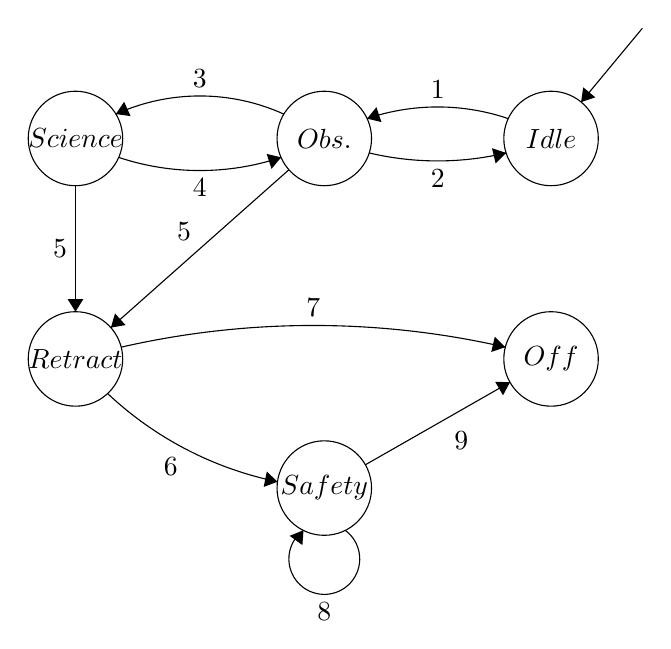
\begin{tikzpicture}[scale=0.2]
\tikzstyle{every node}+=[inner sep=0pt]
\draw [black] (46.2,-13.5) circle (3);
\draw (46.2,-13.5) node {$Idle$};
\draw [black] (31.8,-13.5) circle (3);
\draw (31.8,-13.5) node {$Obs.$};
\draw [black] (16,-13.5) circle (3);
\draw (16,-13.5) node {$Science$};
\draw [black] (16,-27.5) circle (3);
\draw (16,-27.5) node {$Retract$};
\draw [black] (46.2,-27.5) circle (3);
\draw (46.2,-27.5) node {$Off$};
\draw [black] (31.8,-35.7) circle (3);
\draw (31.8,-35.7) node {$Safety$};
\draw [black] (52,-6.5) -- (48.11,-11.19);
\fill [black] (48.11,-11.19) -- (49.01,-10.89) -- (48.24,-10.25);
\draw [black] (34.516,-12.239) arc (108.749:71.251:13.951);
\fill [black] (34.52,-12.24) -- (35.43,-12.46) -- (35.11,-11.51);
\draw (39,-11) node [above] {$1$};
\draw [black] (43.348,-14.419) arc (-76.68931:-103.31069:18.884);
\fill [black] (43.35,-14.42) -- (42.45,-14.12) -- (42.68,-15.09);
\draw (39,-15.43) node [below] {$2$};
\draw [black] (18.564,-11.955) arc (114.4174:65.5826:12.909);
\fill [black] (18.56,-11.95) -- (19.5,-12.08) -- (19.09,-11.17);
\draw (23.9,-10.3) node [above] {$3$};
\draw [black] (29.056,-14.702) arc (-71.60296:-108.39704:16.337);
\fill [black] (29.06,-14.7) -- (28.14,-14.48) -- (28.45,-15.43);
\draw (23.9,-16.04) node [below] {$4$};
\draw [black] (16,-16.5) -- (16,-24.5);
\fill [black] (16,-24.5) -- (16.5,-23.7) -- (15.5,-23.7);
\draw (15.5,-20.5) node [left] {$5$};
\draw [black] (29.55,-15.49) -- (18.25,-25.51);
\fill [black] (18.25,-25.51) -- (19.18,-25.35) -- (18.51,-24.61);
\draw (22.89,-20.01) node [above] {$5$};
\draw [black] (28.83,-35.296) arc (-101.59962:-133.25786:22.283);
\fill [black] (28.83,-35.3) -- (28.15,-34.65) -- (27.95,-35.63);
\draw (22.05,-33.75) node [below] {$6$};
\draw [black] (34.41,-34.22) -- (43.59,-28.98);
\fill [black] (43.59,-28.98) -- (42.65,-28.95) -- (43.15,-29.81);
\draw (40.5,-32.1) node [below] {$9$};
\draw [black] (33.123,-38.38) arc (54:-234:2.25);
\draw (31.8,-42.95) node [below] {$8$};
\fill [black] (30.48,-38.38) -- (29.6,-38.73) -- (30.41,-39.32);
\draw [black] (18.905,-26.751) arc (102.88102:77.11898:54.705);
\fill [black] (43.3,-26.75) -- (42.63,-26.09) -- (42.4,-27.06);
\draw (31.1,-24.87) node [above] {$7$};


\end{tikzpicture}
\end{center}



\begin{center}
Diagram of software states of operation and transition between states [2].

Transitions between states occur as numbered:

\begin{enumerate}
\item{\textbf{Appogee is reached.} The software shall activate when the power line goes to high at 28V. Observation mode shall be 
triggered when the \gls{OBC} turns on. Observation mode will collect a sweep of the payload with the camera. This mode will ensure that the 
camera is operational during the more crticial parts of the mission.}
\item{\textbf{Error: Return to Idle.} If an error is encountered in entering Observation mode, the software shall fallback to Idle 
mode and retry. An error may occur if the payload fails to deploy correctly or if the camera fails to turn on. The system shall send
a signal using the AVR interrupt library if the arm is not fully extended, as the arm is equipped with sensors to determine whether
it is extended or folded. If the camera fails to turn on, the system shall be notified as the telemetry line will be sending empty
data.}
\item{\textbf{Payload Assembly and Camera have been deployed.} The software shall enter Science mode once the payload assembly and arm
 have deployed and the camera has performed an observation sweep. Science mode will consist of the arm touching the sensors in 
 the payload canister, and collecting data via the telemetry line. The whole mode shall be captured with the camera.}
\item{\textbf{Error: Return to Observation} The software shall return to observation mode if any error occurs in Science mode. An error may occur in Science mode if the arm fails to operate correctly and must return to default position. An error may also occur if the camera stops working. The system shall know if the arm fails as a timer can keep track of the time between an arm movement request
and the arm actually completing the movement request. If too much time has elapsed between the request and the movement, the arm may
be stuck. If the telemetry line stops receiving data from the camera, then the camera has stopped working and the system shall be 
notified via an interrupt.}
\item{\textbf{Timer switches to end appogee period.} Once the time period for observation has ended, the timer line will go to low and trigger to Shutdown state. This state can be reached from either Observation or Science mode.}
\item{\textbf{Error: Shutdown not completed successfully.} If an error occurs in the shutdown sequence, the software shall enter Safety mode. An error that could occur is the arm failing to close, the Body failing to retract, or the \gls{OBC} not powering off. All 
these situations except for the \gls{OBC} not powering off are handled through Safety mode.}
\item{\textbf{Retry: Re-attempt to retract the arm.} Attempted to resolve any errors and retry retracting the arm.}
\item{\textbf{Accept: Shutdown correctly} If Shutdown occurs correctly, the arm should be closed, the Arm Assembly Body should be retracted, and the \gls{OBC} should be powered off. The arm will be have sensors to detect whether its closed or not, which can also
be used to know whether it has been retracted into the body. Once the system has determined that this criteria has been met, it
will power off.}
\item{\textbf{Error: Payload is still deployed.} The software shall remain in Safety mode until the payload is either retracted correctly, retracted fully with the arm in the open position, or ejected safely from the rocket. Safety mode shall first try to correctly retract the arm, then retract with the arm open, then repeat attempting ejection until the payload is ejected.}
\item{\textbf{Payload is Shutdown correctly.} If the payload is Shutdown through Safety mode, shutdown can be completed. In Safety mode, the payload was either shut down correctly, retracted fully into the can with the arm open, or the arm was expelled safely from the rocket. The shutdown sequence consists of the arm closing, the Body retracting, and the \gls{OBC} being powered off.}
\end{enumerate}
\end{center}

\subsubsection{Target Success Sensors}
\textbf{Author:} Amber Horvath
\label{subsec:tests}
\subsubsubsection{Requirement Overview}
The software shall know whether or not the arm succeeded in touching the targets generated, as described in subsection 2.1. The sensors
shall report back whether or not contact was made. This data can be used in post-mortem analysis to determine whether
certain targets were faulty or whether the range of motion on the arm was faulty.
\subsubsubsection{Solution Design}
The payload shall be equipped with pre-placed sensors that the arm shall make contact with. The arm shall have generated targets
as described in subsection 2.1. These coordinates shall be stored within the system and used as inputs for the function controlling
the arms' movements, with the target position being where the tip of the arm should be located. The arm shall exert force to touch
the sensor, and the sensor shall go high if contact is made. The sensors high or low signal shall be sent via the telemetry
line and written to our SD card. If the arm gets stuck during this process, it will enter Safety mode, as described in subsection 2.5. The telemetry data shall
later be visualized using Python's UI package, TK. 

\subsubsection{Telemetry}
\textbf{Author:} Michael Humphrey
\subsubsubsection{Requirement Overview}
The telemetry component shall report via telemetry all error codes and test results.

\subsubsubsection{Solution Design}
The telemetry component is responsible for collecting and sending data through the
telemetry ports on the \gls{payload}.

This component shall not be responsible for transmitting data generated from the
temperature sensors.
The temperature sensors will be wired directly to an analog telemetry port,
bypassing the \gls{OBC} altogether.

For each test the software successfully completes (see \hyperref[subsec:tests]{subsection 
\ref*{subsec:tests},  Target Success Sensors}) this component shall output a code
representing the test number to the telemetry port.
There shall be two tests; one for each touch point on the \gls{payload}.
The tests shall be designed as a joint effort between the Hephaestus Structures,
Robotics, Electrical, and Software teams.

The output shall be encoded as a four character \gls{binstring} and transmitted
simultaneously via a four parallel port pins.
The \gls{binstring} shall be transmitted at a rate of no more than 5,000 Hz.
There shall be a delay of no less than .2 milliseconds between transmissions
of codes.
When no code is being actively transmitted, the telemetry shall output a code
of `0000' to the telemetry pins.

In addition to transmitting codes via the telemetry lines, the software shall also
store a log file with timestamps on an onboard SD card.
The log file shall consist of a series of lines of text, consisting of a timestamp
and a description.
The timestamp shall be the number of tenths of milliseconds since the \gls{OBC}
powered on.
The description shall be a sequence of \gls{ASCII} characters of arbitrary length,
and terminated with a carriage return character.

\subsubsection{Video Handling}
\textbf{Author:} Michael Humphrey
\subsubsubsection{Requirement Overview}
Video footage of the \gls{payload}'s operations shall be recorded and saved to the
SD card.

\subsubsubsection{Solution Design}
The Hephaestus Electrical Engineering team shall design the payload such that the 
camera will power on and off at the appropriate times, as well as save footage to
the SD card. 

\subsubsection{Data Visualization and Processing}
\textbf{Author:} Michael Humphrey
\subsubsubsection{Requirement Overview}
The data visualization and processing component shall provide visualizations
for the collected data.
This component shall be able to show whether the mission success criteria have
been met or not.
If the mission success criteria have not been met, this component shall show how
and why they have not been met.

\subsubsubsection{Solution Design}
The component shall have a \gls{gui} written in Tkinter with graphs generated by
\gls{matplotlib}.
The \gls{gui} shall consist of two graphs, a table, and a timeline.
Each graph shall be a \gls{plot} with analog data collected from each of two temperature sensors.
The data from the temperature sensors shall be graphed with respect to time from
\gls{apogee} and actual temperature, if such a value can be determined.
In the absence of a method to reliably determine actual temperature from the raw
sensor data, then the data shall be graphed with respect to the raw value received
from the sensor, with the graph scaled such that the lowest value recorded shall be
the minimum y value, and the highest recorded value recorded shall be the maximum y value.
The user shall be able to scale the graphs to view portions of the data as they see fit.
The table shall consist of the name of each of a series of tests,
the result of that respective test, and the time that test was completed.
A result shall be either ``passed'', ``failed'', or ``not completed''.
A result of ``passed'' shall be colored in green.
A result of ``failed'' shall be colored in red.
A result of ``not completed'' shall be colored in yellow.
If the result of a test is ``not completed'', then the time of completion for that test
may be omitted.
There shall be two total tests.
The tests shall be for if the \gls{payload} can successfully touch each touch point sensor.
The tests shall be designed as a joint effort between the Hephaestus Structures,
Robotics, Electrical, and Software teams.
The timeline shall be a visualization with time on the y axis, with significant events
marked at various positions along the axis, according to when that event happened.


\subsection{Conclusion}
This concludes the design of our project. Further questions or concerns can be addressed to the authors of this document.
This document may be subject to changes in the future as more design constraints are found, or designs are found to not work the way


\subsection{Changes Since Original Design Document}

\section{Technical Review Document}
\subsection{Original Technical Review Document}
\input{OrigTechRevDoc.tex}
\subsection{Changes Since Original Technical Review Document}

\section{Weekly Blog Posts}
NOTE:Follow the format and put your posts for fall week 4 in Fall 2016/Week 4/Your-Name for example. Change the weeks to have the right ranges. Delete this note.

\subsection{Fall 2016}
\subsubsection{Week 3}
\subsubsubsection{Helena Bales}
\textbf{Progress} \\
This week I made significant strides in the design of our project. I wrote part of the Project Definition assignment. I started the Project Description with a description of the problem, broken down into the requirements of the RockSat-X program and the payload that we decided on for the project. In order for our senior design project to be successful, we have to build the payload, meet the RockSat-X project requirements (such as testing, documentation, and design reviews), and meet the capstone class requirements. Our payload idea is a mechanical arm, and as a project it is capable of meeting all the requirements.

While the Project Definition document met our capstone class requirements for the week, there were also RockSat-X requirements to be met this week. The RockSat-X CoDR (Conceptual Design Review) was this week. As a large group (including two teams of ME's, one team of EE's, and the CS team) we developed the CoDR powerpoint that was presented yesterday to RockSat-X. This document included all of our conceptual payload designs thus far, and was our first time presenting our designs to the RockSat-X group. Following that presentation, in order to meet the RockSat-X requirements, we took a group photo.

In addition to the RockSat-X requirements and the capstone class requirements, we met the payload requirements by meeting with Nancy Squires to discuss the project, get approval of the Project Definition assignment, and discuss starting an official Space Lab at OSU.

\textbf{Plans} \\
The next week will be focusing on the development of documents for Senior Design class as well as for the RockSat-X project. Specifically, we will be revising the Project Description document and begin the Requirements Document. We will also be continuing the design process for the payload with the other teams.

\textbf{Problems} \\
The problems that we have encountered have been minimal so far.

\subsubsubsection{Amber Horvath}
\subsubsubsection{Michael Humphrey}
\textbf{Progress} \\
This past week the Hephaestus project team accomplished several important milestones. We completed our first presentation to the RockSat-X organizers and took a group picture to start raising funding. We are also starting to narrow down our design for the final \gls{payload}.

\textbf{Plans} \\
Because the mechanical and electrical design of the project is not yet finalized, the software team has not yet had any important responsibilities. The electrical team is forbidden from using a device like a Raspberry Pi or an Arduino, so they have decided to use an AVR microcontroller. Amber and I have not used one of these devices, although Helena has. Amber and I will need to start doing research on programming for these devices. We will be using C to program the microcontroller. We won't be able to write any code until the electrical design (i.e. inputs and outputs) are finalized, but we can start creating a software design of how we want the software to work.

\textbf{Problems} \\
No problems have been encountered yet.

\subsubsection{Week 4}
\subsubsubsection{Helena Bales}
\textbf{Progress} \\
This week I was at the Grace Hopper Celebration of Women in Computing. I did not do any work directly on the RockSat-X project, but I did talk to many people about Computer Science and space exploration.

\textbf{Plans} \\
Next week will be focusing on the development of the requirements document for Senior Design and PDR presentation. The PDR presentation is coming up and will require us to compile a powerpoint about our design, practice presenting it, and presenting it for the RockSat-X program.

\textbf{Problems} \\
I encountered a significant obstacle to completing work this week. I did not have internet access at Grace Hopper, so I was unable to work on the project or create an update.

\subsubsubsection{Amber Horvath}
\subsubsubsection{Michael Humphrey}
\textbf{Progress} \\
Similar to week 3's blog post, this past week the Hephaestus Software Team did not have any major responsibilities. We attended the Hephaestus team meetings where the mechanical and electrical designs are still being worked out. We are going to have more communication with the Electrical Engineering team to determine the computing platform and computation restrictions. We also began working out budget numbers.

\textbf{Plans} \\
This next week we will be creating several presentations. I will be partly responsible for a 6 minute 40 second presentation to compete for a \$1,000 cash prize. Other fundraising efforts are also in progress. We will also be meeting with the Colorado Space Grant committee for our next presentation for them. We will also need to start working on revising our Problem Statement and start drafting our Requirements document and any other documentation we need.

\textbf{Problems} \\
Currently, the software team is blocked by the electrical team. Until they finalize a design, we cannot start coding. We will be in communication with them, however, to determine what considerations they need to take for the design.

\subsubsection{Week 5}
\subsubsubsection{Helena Bales}
\textbf{Progress} \\
This week was focused on developing the requirements document for Hephaestus and revising the Project Description document. The revision of the Project Description document was turned in on Wednesday after adding more of a focus on the software side of the project. The first draft of the requirements document will be turned in by the end of the day today. I focused on creating the outline of the document and writing the introduction. The introduction establishes a purpose and description of the document, an overview of the mission description, the mission success criteria, and the priorities for the requirements. The rest of the document describes the functional and non functional requirements that we have established for the software that controls the Hephaestus payload.

\textbf{Plans} \\
The next week will focus on creating a solid final draft of the Requirements Document and presenting PDR. That will require meeting as a group to practice presenting PDR and meeting as a group to present PDR.

\textbf{Problems} \\
Availability has been a problem this week. It has been a challenge to fit all of the large group meetings into my schedule and still have time to catch up on homework after Grace Hopper and work.

\subsubsubsection{Amber Horvath}
\subsubsubsection{Michael Humphrey}
\textbf{Progress} \\
Since our mechanical and electrical design is still in progress, we have made no progress in the past week toward writing any software. Only work done was finishing the problem statement assignment and drafting our requirements document.

\textbf{Plans} \\
For the next week we will be getting datasheets and other information from the electrical team to aid in drafting our requirements documents. Any limitations of the hardware will be taken into consideration for the software requirements. Those materials should be made available by the electrical team by early next week.

\textbf{Problems}
Problems encountered this week were mostly personnel issues. Some of our team has been on vacation and one member is now sick and unable to make it on campus at all. I feel myself coming down with my second illness this term, which will make it even more difficult to get the required signatures we need.

\subsubsection{Week 6}
\subsubsubsection{Helena Bales}
\textbf{Progress} \\
This week, work focused on the development of the Requirements Document for Senior Design and finalizing the PDR presentation for RockSat-X. I mainly focused on the Requirements Document, and did significant work on the structure and content of that document. We turned in a draft first, then flushed it out to a final document that was turned in on Friday of Week 6. I focused on the functional requirements, introduction, and structure of the paper. For the PDR presentation, we had to develop requirements and a plan to meet the requirements. There was a lot of overlap in content between PDR and the Requirements Documents, which was ideal for finishing both of these big documents in the same week. In preparation for this presentation, we had one meeting where we all went over content and one where we practiced the presentation. The final presentation for PDR (Preliminary Design Review) was at 7am on Thursday of week 6. Finally, I revised the README for this repository, so that it was more informative regarding the structure, contents, and context of this repository.

\textbf{Plans} \\
Next week will focus on finalizing major design choices and developing the technical review. The design choices that need to be finalized include the method for assigning test points and the operational modes of the arm.

\textbf{Problems} \\
None.

\subsubsubsection{Amber Horvath}
\subsubsubsection{Michael Humphrey}
\textbf{Progress} \\
This week was spent finalizing our software requirements for the project. We did extensive research into the details of the mechanical and electrical design of our \gls{payload} and drew up documents with specifics such as coordinate systems and \gls{payload} layout. We now have a basis for creating our software.

\textbf{Plans} \\
For the next week, I believe we will be able to start writing the framework for the \gls{payload}. We probably won't be able to start programming the actual function of the \gls{payload} until it is built, but we can create the structure of how our software will be laid out.

\textbf{Problems} \\
Some problems were encountered this week with communication outside of our sub-team, but those have been resolved and shouldn't occur again in the future.

\subsubsection{Week 7}
\subsubsubsection{Helena Bales}
\textbf{Progress} \\
This week we are developing the Technical Review Document for Senior Design. As such, we have divided the requirements up between the three of us as follows:

\textbf{Amber Horvath:}

    Emergency Expelling of Payload

    Program Modes of Operation

    Target Success Sensors

\textbf{Helena Bales:}

    Target Generation

    Movement of arm

    Arm position tracking

\textbf{Michael Humphrey:}

    Telemetry

    Video Camera

    Data visualization and processing

Each of us shall be responsible for insuring the completion of their assigned tasks. We will focus on our assigned tasks for the tech review. This week has focused on defining and assigning the requirements to each of us. We have also finalized some design choices, specifically in the modes of operations, emergency procedures, and arm target generation.

\textbf{Plans} \\
Next week we will complete and turn in the tech review on Monday of Week 8. Before that date we will be finishing that document. After the completion of the tech review we will be going back through past documents and including all suggestions we have received as feedback throughout the course. We will be doing this to prepare for the final document to be turned in on December 4th. We will also be preparing our designs and requirements for our big RockSat-X review during weeks 10 or 11.

\textbf{Problems} \\
We mainly are encountering the issue that we have too many assignments due on or before Monday of Week 8.

\subsubsubsection{Amber Horvath}
\subsubsubsection{Michael Humphrey}
\textbf{Progress} \\
Last week we developed the requirements of our system a lot. We explored technologies that we want to use and confirmed many details with the robotics and electronics team about the requirements of the \gls{payload}. For me, last week was spent primarily going to meetings, relaying information to teammates, and doing research into potential technologies we can use.

\textbf{Plans} \\
Next week, we will hopefully begin implementation of the software. I need to set up a meeting with the electrical team. I can't remember what they want to talk about but we definitely meet as a team with them. Most likely all of the CS team won't be able to make it, and this is a challenge we will need to overcome.

\textbf{Problems} \\
Problems I encountered included finding adequate solutions for the telemetry technology. I thought it would be easy to find several solutions we could use, but it turns out that most of the solutions I found were not compatible with our system for one reason or another. Mostly because none of them actually dealt with the transmission of the data itself, but what it did with the telemetry after it was collected. Other reasons were that they were implemented in the wrong language.

\subsubsection{Week 8}
\subsubsubsection{Helena Bales}
\textbf{Progress} \\
This week we finalized and turned in the technical review document. Preparing this document required meeting as a group to talk about potential solutions, then documenting the solutions that we came up with. This week we also talked to the Electrical Engineering group to make sure that our plans were consistent and that we would be able to work together on the software/hardware interface in the future.

\textbf{Plans} \\
Next week we plan on starting the Design Document and the presentation for the end of the term and our CDR presentation with RockSat-X.

\textbf{Problems} \\
I have been experiencing technical issues with my computers, so that is something that I will need to resolve before I can seriously start working on the Design Document.

\subsubsubsection{Amber Horvath}
\subsubsubsection{Michael Humphrey}
\textbf{Progress} \\
Last week I helped start our Design Document. We've created the structure for the document and pasted the relevant sections from our previous documents. I set up meetings with the Electrical team and started communication with them to nail down specific software communication requirements. They're going to create a sort of "firmware" for the \gls{payload}, meaning they'll write the code that interacts directly with the hardware, and they'll expose an abstract interface for the Software team so we only need to call something like moveArm(x, y, z); to control the movement of the arm.

\textbf{Plans} \\
Next week we need to finalize the details of how we want to control the \gls{payload} arm. This will probably mean writing an API that we want the Electrical team to implement. We also need to prepare for the CDR coming up in a couple of weeks. This means we need to fill out the slides the Software team is responsible for. There will probably be other work for this presentation that we will tackle as it comes up.

\textbf{Problems} \\
No problems this week.

\subsubsection{Week 9}
\subsubsubsection{Helena Bales}
\textbf{Progress} \\ 
This week we started the Design Document and slides for the presentation for this class and for our RockSat-X program CDR. We met in order to discuss the solutions that we wanted to choose for each of the requirements. During that meeting I updated our Design Document to reflect the choices that we made, and created issues to reflect the tasks that we have yet to complete.

\textbf{Plans} \\ 
In the next week we will be finishing the Design Document, finishing our slides for the class presentation, finishing our slides for the CDR presentation, practicing the CDR presentation, and starting to compile the progress update assignment.

\textbf{Problems} \\ 
I am still experiencing technical issues with my computer, but less seriously than before, so progress has been made there.

\subsubsubsection{Amber Horvath}
\subsubsubsection{Michael Humphrey}
\textbf{Progress} \\
This week I didn't do much. The Software team has created an outline for our design document but I haven't added my parts in. I don't foresee it being too much work, as it's mostly already written from the tech review. More details just need to be added. Due to it being Thanksgiving week, I have delayed working on classwork in favor of helping my family prepare for Thanksgiving.

\textbf{Plans} \\
Next week we need to finish our rough draft of the design document as well as write an outline for our presentation.

\textbf{Problems} \\
No problems were encountered this week.

\subsubsection{Week 10}
\subsubsubsection{Helena Bales}
\textbf{Progress} \\ 
This week we finished up the Design Document and started the Progress Update write up and presentation. We also prepared for CDR by adding slides to the presentation. In order to finish the design document we talked about how to solve each of the issues from the Requirements document. Once we picked a solution to pursue, we each added detail to our solutions. The CDR presentation was adapted to form the start of our Progress Update presentation since it already describes the project and our work thus far.

\textbf{Plans} \\ 
Next week we will be finishing our progress update write up and presentation. We will do the write up first, then make sure that the presentation slides cover the content from the write up, and finally record the presentation.

\textbf{Problems} \\ 
None.

\subsubsubsection{Amber Horvath}
\subsubsubsection{Michael Humphrey}
\textbf{Progress} \\
This week we made a lot of progress finalizing the design for the \gls{payload} software. This was mostly a result of writing the design document. There was much communication with the electrical team.

\textbf{Plans} \\
Next week is finals week. We will be writing our progress report and recording our presentation.

\textbf{Problems} \\
One problem we are encountered is the slow response to questions that arise about the RockSat-X program. I have several questions about the format and delivery of telemetry data that won't be answered until mid- to late-next week. That information was not able to be included in the design document.


\subsection{Winter 2017}
\subsubsection{Week 1}
\subsubsubsection{Helena Bales}
\textbf{Progress} \\ 
I made no progress over winter break, other than actually managing to take a vacation. I am very proud of myself.

Since the start of week 1, I met with the Software Team to discuss the schedule that we will have for the term. We decided that we would have an hour long meeting on Mondays after our TA meeting and an hour long meeting with the whole Hephaestus team on Thursdays at 6pm. We have not yet had a Monday meeting because the past two mondays have been cancelled due to weather and MLK Day.

We accomplished some tasks for week 1, which includes adding more content to the System Architecture for the Software Subsystem. In addition to this planning I began development of the test cases that will be used to test the Software Subsystem. Specifically, I am focusing on developing experiments to test the three functional requirements that I was assigned last term.

\textbf{Plans} \\ 
The plan for next week is to finish up the architecture diagram and the test cases and beginning the implementation phase of the project. We need to have a prototype completed and tested by mid February, so we are planning on implementing for three weeks then testing.

\textbf{Problems} \\ 
My biggest problem is that I do not have a working computer right now. I have been trying to fix my computer but it has just been a time sink so far. I don't have a solution to this problem.

\subsubsubsection{Amber Horvath}
\subsubsubsection{Michael Humphrey}
\subsubsection{Week 3}
\subsubsubsection{Helena Bales}
\textbf{Progress} \\ 
This week we started really diving into the motion planning in the Pathing and Automation cross-functional team. I checked out books from the library to help with research into motion planning for robotics, robotics in space, and inverse kinematics.

\textbf{Plans} \\ 
Over the next weeks I will be doing research into the issues of path planning and motion tracking on earth and in space.

\textbf{Problems} \\ 
I still don't have a working computer with which to do the research.

\subsubsubsection{Amber Horvath}
\subsubsubsection{Michael Humphrey}
This is a cumulative update for the first three weeks of Winter term.

\textbf{Progress} \\
The progress we've made up to this point includes installing Atmel Studio, 
setting up a solution for our class, and setting up several skeleton files. 
I've created a file for the first phase of the program; the idle phase. It is 
mostly filled out except for the code to interface with the pin. I've also set
up a file in our Google Drive detailing rules and instructions for laying out 
our project and how we will develop. We also had a meeting with the EEs about 
any telemetry data they need transmitted. They reported that they have no 
special need for transmitting telemetry via the microcontroller (all the data 
they need will be hard-wired to the telemetry interface), so I can freely 
design and implement the telemetry code without any outside interference.

\textbf{Plans} \\
My plan for the next week is to become up to speed with the driver and 
interface that the EE team has created for us, so that I can begin full-time 
development on the project. I plan to finish designing and start implementing 
the telemetry code, as well as finalize the idle phase of the code.

\textbf{Problems} \\
Problems I encountered these first few weeks include waiting for the EEs to 
develop the motor drivers and telemetry interface. Other problems include team
members not showing up to cross-functional team meetings, so we couldn't get 
information on how to use the drivers and interface. We had to schedule a 
special meeting much later with the EEs so we can start using the code they 
wrote.

\subsubsection{Week 4}
\subsubsubsection{Helena Bales}
\textbf{Progress} \\ 
This week was continuing research into the pathing and automation portion of the software. I have found that the A* algorithm for pathfinding within a configuration space will be a good solution. Additionally, we will be breaking up the arm into its individual links in order to move the arm to a valid configuration. Essentially, we will start at the base of the arm and move that first, then move up the arm to the next link and move that.

\textbf{Plans} \\ 
The next week will be finishing up the research phase for pathing and automation and starting implementations. We will be starting with building the Configuration Space.

\textbf{Problems} \\ 
We still haven't figured out a good way to build a C-Space.

\subsubsubsection{Amber Horvath}
\subsubsubsection{Michael Humphrey}
\textbf{Progress} \\
This week I hit a major personal milestone for this project. I finally was 
able to compile the (mostly useless) code we've all written so far this term 
and run it on the actual microcontroller! It compiled successfully for me, and
although it didn't do much it was a relief to see the fruits of our labor to 
work. The code did not compile on Amber's computer, but that was probably 
because she is using a mac and mac's are not directly supported by the avr 
compiler. I helped her troubleshoot a little bit, but she eventually figured 
it out on her own. I also added to our Description of Operations to detail 
more about the telemetry codes. Other than that, this week was spent waiting 
for drivers from the EE team for motors and pin inputs.

\textbf{Plans} \\
My plan for the next 
week is to create some constants in the telemetry header file that will encode
telemetry codes as well as constants for telemetry operation (such as the 
length of time codes will be broadcasted).

\textbf{Problems} \\
No problems encountered.

\subsubsection{Week 5}
\subsubsubsection{Helena Bales}
\textbf{Progress} \\ 
This week was focusing on figuring out how to build the configuration space (C-Space) in which to perform the path-finding algorithm for the arm's motion. We found that the C-Space need to be in \(R^4\) because we have 4 degrees of freedom in the arm. We also know that for each possible configuration of the arms' motors, we need to know if the configuration is valid in order to map the C-Space. This week we are also starting on the slide for STR.

\textbf{Plans} \\ 
The next week will focus on finalizing the slides for STR. Our STR presentation will be at 6am on Friday of week 6. In addition to STR, the Pathing and Automation and Software groups will be meeting with Dr. Smart during week 6 to discuss methods for building the configuration space.

\textbf{Problems} \\ 
I am blocked from progressing further with the code for motion planning because we do not yet know enough about the C-Space and how to build it. This should be resolved next week after meeting with Dr. Smart.

\subsubsubsection{Amber Horvath}
\subsubsubsection{Michael Humphrey}
\textbf{Progress} \\
This week I updated my three sections of the design document. Additionally, I 
reviewed the tech and requirements, but no changes were required to either of 
these documents. Additionally, I met with our TA to review feedback on these 
documents last time they were graded, but there was not much feedback. I 
communicated the feedback there was to the rest of the team.

\textbf{Plans} \\
For the next week, I hope to finish the idle phase by implementing the flags 
provided in the drivers. Additionally, I would like to complete writing 
definitions for codes in the telemetry header file.

\textbf{Problems} \\
No problems encountered.

\subsubsection{Week 6}
\subsubsubsection{Helena Bales}
\textbf{Progress} \\ 
This week involved finishing the presentation for STR, a all-team social event, presenting STR, and meeting with Dr. Smart. The meeting with Dr. Smart was on Monday and provided a lot of useful information for pathfinding and automation. We discussed methods for creating the Configuration Space. Dr. Smart explained the ways in which we should limit the payload to keep the configuration space as a plane in R4. We also discussed the best way to generate the configuration space. The options that we discussed were calculating it mathematically using Inverse Kinematics, running a simulation in solid works, or physically moving the arm to valid configurations and mapping those. Each of these methods has benefits and drawbacks. STR occured on friday. In preparation we created the slides throughout the week. On thursday, at our all-team meeting, we went through all the slides in preparation for the presentation on Friday at 6am. The presentation went very well on Friday. The project reviewer said that she was excited to see our project and that our presentation and progress were both very good. The all-team social was at the All-Team meeting on Thursday after we finished all relevant business. We ordered pizza and played board games. The Software team was divided between the two teams with Michael and I against Amber. Amber's team won the first two rounds, but Michael and I brought in a win in the last round. All in all, it was an effective evening of work and team bonding.

\textbf{Plans} \\ 
The next week will focus on creating and recording our presentation for the Senior Design class. We will be working on the presentation on Tuesday, finishing it on Wednesday in order to record the video on Wednesday or Thursday. We will finish the project with editing and posting the video on Thursday and Friday to have it done by Friday. I will also be updating the design documents from last term to reflect the changes we have made. I do not expect there to be significant changes, however there may be some slight modifications to the pathfinding and automation section to reflect what Dr. Smart taught us this week.

\textbf{Problems} \\ 
The motors have arrived, so I am no longer blocked on progressing in the code. Following the completion of the presentation for CS462, I will be able to dive into the pathfinding code.

\subsubsubsection{Amber Horvath}
\subsubsubsection{Michael Humphrey}
\textbf{Progress} \\
The bulk of this week's work was spent editing the software slides for the STR
presentation. In addition to this, I implemented the remaining portions of the
idle phase code and sat in on a meeting with Dr. Smart about robotic arm 
movement and pathing. From that I have a much better idea on how the pathing 
algorithm will work.

\textbf{Plans} \\
My plan for next week will be slightly smaller in scope due to personal 
obligations. However, I will make sure my portions of the requirements and 
design documents are up to date and that we're on track to complete the 
assignment we received an extension on. I also plan on finally completing the 
telemetry header file, as well as signing up our team for the expo.

\textbf{Problems} \\
Nothing currently blocking.

\subsubsection{Week 7}
\subsubsubsection{Helena Bales}
\textbf{Progress} \\ 
This week was focused on preparing the Midterm project update for the Senior Design course. I started the slides on Monday using our STR presentation as a base and added more details on the software side of the project and deleted many of the slides from STR that were focused on the hardware side. On Thursday we met as a group to finalize the slides and record the audio. Michael then edited the audio while I worked on updating our written documents for last term, compiling my blog posts, and starting the retrospective. Also on Thursday was the all-team meeting. We discussed funding issues because AIAA will not be contributing as much money to the project as they initially said they would, so we now have about \$30,000 to fund raise. We will all be reaching out to previous employers, etc. to raise the remainder of the funds.

\textbf{Plans} \\ 
The next week will focus on building the configuration space. We are still trying to get motors to use for this step since they need to be back-driven and have encoders. We will be buying foam to line the payload. We will then line the payload with foam to provide a buffer of forbidden space in the C-Space before any collision occurs between the arm and payload. Next we will attach the motors to the arm and an arduino. We will use the arduino to read values from the motors as we back-drive them through every valid configuration. Finally, we will use this data to build the c-space. This will take up most of the week. The only other plan is that the Tuesday Senior Design class is required attendance.

\textbf{Problems} \\ 
We have not yet found motors to use for building the C-Space.

\subsubsubsection{Amber Horvath}
\subsubsubsection{Michael Humphrey}
\textbf{Progress} \\
This week I have made absolutely no progress. I have been kept busy with grad 
school application and other personal issues. Progress will resume after March
1st.

\textbf{Plans} \\
Goal for next week is start writing telemetry header file.ash

\textbf{Problems} \\
No issues.

\subsubsection{Week 8}
\subsubsubsection{Helena Bales}
\textbf{Progress} \\ 
This week was focused on preparing the payload to build the configuration space. On Tuesday I went to the required Senior Design class. I wrote and practiced pitching and talking about the Hephaestus project. After class I talked to McGrath about getting motors with encoders to build the Configuration Space. He gave us three motors that we can back-drive and hook up to an arduino. Later in the day on Tuesday I worked with the Pathfinding and Automation team to prepare the payload to build the C-Space. I bought foam board and cut out pieces of it to line the payload. With this complete, we need to attach the motors to the arm and the arduino then read the values from the motor.

\textbf{Plans} \\ 
The next week will mostly be working on the C-Space more and the arm control software. I will be starting by writing arduino code that we can use to build the C-Space. I will be working on that this weekend. Once that is complete, we will build the C-Space. After we have the C-Space, I will start the arm control software that will plot the path through the C-Space and move the arm along the path.

\textbf{Problems} \\ 
None.

\subsubsubsection{Amber Horvath}
\subsubsubsection{Michael Humphrey}
\textbf{Progress} \\
Not much progress this week. Can't develop without a prototype to test on. 
Can't write code if we can't run it. (I mean we could but that would be a 
colossally awful idea.)

\textbf{Plans} \\
Plan for next week is to design and begin implementation of motor test. This 
test (or tests) won't be used during the payload deployment on the rocket, but 
they will be used to demonstrate the payload actually works on earth, for 
various design requirements.

\textbf{Problems} \\
Only problems are that the Pathing team is hogging the only working prototype.

\subsubsection{Week 9}
\subsubsubsection{Helena Bales}
\textbf{Progress} \\ 
My primary goal this week was to get an initial mapping of the C-Space. I met this goal. On Tuesday I met with Pathing and Automation to start work on the Arduino code to map the C-Space. They had a start to it with three motors on interrupts and printing their values to Serial out. Unfortunately, the Arduino UNO only has two interrupt pins, so I had to switch one of the motors to poll instead of interrupt. This took a few tries, but by Thursday, which is when we met next, I had a motor polling instead of interrupting. I had also fixed the print statements to be more useful to us. However the code still had some bugs. We ran out of time on Thursday and had to go to the All-Team meeting, so we met up the next day as well. On Friday I finished debugging the Arduino code and we were finally ready to map the C-Space. I ran the arm all around the payload so we now have an initial data set on the shape of the C-Space to play with.

\textbf{Plans} \\ 
My next step in the software is to write a parser for the C-Space data. It is currently in the form of one motor angle per line, with the triples separated by a line with a semicolon on it. So I will go from:

\[ theta1 theta2 theta3 ;\]

to:

\[ point_n = <0, theta1, theta2, theta3> \]

I will have a 4D array of 1's, then fill in a 0 in every location indicated by point\_n above. The 4D C-Space will then contain a 0 for every valid configuration of motors and a 1 for every invalid configuration.

Once I have an initial C-Space, I will need to do some repair on it to smooth out the C-Space. This will account for angles that are valid but were not sampled.

My other goal for Week 10 is to help the ME's test the payload. They are all finishing up their capstone class, so they need to have a bunch of tests done to show that their parts of the project work. They will need some help from CS and EE in order to test how their hardware parts all work in motion. I will be helping them to write code to move the arm and to devise test cases.


\textbf{Problems} \\ 
I currently have way too many projects going on. All of my classes have final projects, so I am worried that I will not have time to get it all done.

\subsubsubsection{Amber Horvath}
\subsubsubsection{Michael Humphrey}
\textbf{Progress} \\
This week I worked with Jonathan Hardman from the electrical team to create a 
test program to run the arm. It operates each motor individually to 
demonstrate its full range of motion. The Robots team said they needed the 
file as soon as possible, so I dropped everything to make it. They did not end
up using it.

\textbf{Plans} \\
Next week I plan on working on the slides for our next big presentation, 
Integrated Subsystem Test Review. It is on Friday of finals week. I also plan 
to do the majority of the work for the final presentation and report for this 
class.

\textbf{Problems} \\
Nothing blocking.

\subsubsection{Week 10}
\subsubsubsection{Helena Bales}
\textbf{Progress} \\ 
This week has been an extremely stressful one. All of my classes have final projects. I have not had time to write the parser for the C-Space data. I did update the presentation for the Final Update video. I have some more visuals to add, but I have recorded most of my audio.

We are also working on the presentation today. We did not realize that it was due tonight, so we will be getting most of it done at 4pm today. Needless to say, we are are stressed by this looming deadline.

\textbf{Plans} \\ 
Configuration Space: \\ 
My next step in the software is still to write a parser for the C-Space data. It is currently in the form of one motor angle per line, with the triples separated by a line with a semicolon on it. So I will go from:

\[ theta1 theta2 theta3 ; \]

to:

\[ point_n = <0, theta1, theta2, theta3> \]

I will have a 4D array of 1's, then fill in a 0 in every location indicated by point\_n above. The 4D C-Space will then contain a 0 for every valid configuration of motors and a 1 for every invalid configuration.

Once I have an initial C-Space, I will need to do some repair on it to smooth out the C-Space. This will account for angles that are valid but were not sampled.

Fundraising: \\ 
My other goal for Finals Week is to contact people to ask for funding for our project. We also have ISTR on Friday of Finals week, so we will be spending some time during Finals week working on the presentation for that. We will also be finishing up our presentation and video for this class.

Expo Poster: \\ 
Finally, we will be completing the Expo poster next week as we got an extension from Kirsten. I have defined the general sections on the poster in the poster template. This will cover the sections of the poster, the images on the poster, and the assignments for text and graphics.

Poster Sections: \\
\begin{enumerate}
\item{Panel 1 - Achieving Detailed Autonomous Movement in Space}
\item{Panel 1 - a - Building the Configuration Space}
\item{Panel 1 - a - i - Creating the Configuration Space from Real Space Data}
\item{Panel 1 - b - Pathfinding in an IR 4 Configuration Space}
\item{Panel 1 - b - i - Dijkstra's Algorithm}
\item{Panel 1 - c - Accuracy and Obstacle Avoidance}
\item{Panel 1 - c - i - Accuracy}
\item{Panel 1 - c - ii - Obstacle Avoidance}
\item{Panel 2 - A Rocket-Mounted Autonomous Robotic Arm for Construction in Space}
\item{Panel 2 - a - Hephaestus Mission}
\item{Panel 2 - b - Mission Success Criteria}
\item{Panel 2 - b - i - Minimum Success Criteria}
\item{Panel 2 - b - ii - Maximum Success Criteria}
\item{Panel 2 - c - i - Overview}
\item{Panel 2 - c - ii - Telemetry}
\item{Panel 2 - c - iii - Data Storage}
\item{Panel 3 - Programmatics}
\item{Panel 3 - a - Launch Details}
\item{Panel 3 - b - Sponsors}
\end{enumerate}

Section Assignments: \\
\begin{enumerate}
\item{1 - Helena}
\item{2 - a - Amber}
\item{2 - b - Amber}
\item{2 - c - i - Michael and Amber}
\item{2 - c - ii - Michael}
\item{2 - c - iii - Amber}
\item{3 - a - Michael}
\item{3 - b - Michael}
\end{enumerate}

Images: \\ 
\begin{enumerate}
\item{1 - Landscape - Pathfinding through IR4 Graphic}
\item{2 - Landscape - Hephaestus Payload}
\item{3 - Portrait - ???}
\item{4 - Landscape - Team Photo}
\end{enumerate}

Image Assignments: \\ 
\begin{enumerate}
\item{1 - Helena}
\item{2 - Amber}
\item{3 - Amber/Michael}
\item{4 - Michael}
\end{enumerate}

\textbf{Problems} \\ 
I currently have way too many projects going on. All of my classes have final projects, so I am worried that I will not have time to get it all done. Additionally, I feel the stress of the end of the term is affecting the effectiveness of our team. Spring break will help with that.

\subsubsubsection{Amber Horvath}
\subsubsubsection{Michael Humphrey}
\textbf{Progress} \\
This week I developed an application to read data from a file (ostensibly 
temperature data from a file on the on-board SD card) and display a graph of 
that data. This program is a prototype for our final application to fulfill 
the Data Visualization component of the requirements. The program is a Python 
script with the graph created using the matplotlib library. The program was 
made now to help the Electrical team fulfill a requirement for their senior 
design class.

In addition to the program described above to display the data file, I created
a helper program (also in Python) to generate the data file with random data. 
The temperature sensor that will generate the data only produces 10-bit 
values, so the random data generator must simulate that output. The program 
generates a random value between 0 and 1,023 (inclusive) and outputs it as a 
two byte sequence to a file specified in the arguments to the script. The 
program repeats this 100 times, outputting a null byte (0) as a separator 
between each value. This file can then be used as an input file for the data 
processing program.

\textbf{Plans} \\
Next week will be spent working on the senior design report and presentation. 

\textbf{Problems} \\
Nothing blocking. 


\subsection{Spring 2017}
\subsubsection{Week 1}
\subsubsubsection{Helena Bales}
\textbf{Progress} \\
This week was a light one for Senior Design. I attended the first class on Wednesday and met with my group and the TA on Tuesday. Both meetings gave me an overview of the deadlines and expectations for this term. I met with the whole RockSat-X group on Wednesday for a meeting, pizza, and games. The other team members kept calling me Amber. We did not have a pathing and automation cross-functional group meeting this week since we didn't figure out scheduling soon enough. I did some work on the Parser for the C-Space.

\textbf{Plans} \\ 
I plan to finish the C-Space parser next week and move on to pathfinding. I will also be making some funding requests so that we can hopefully travel to the integration testing and launch.

\textbf{Problems} \\ 
The main problem for this week is a funding shortage that may mean that we will not be able to send everyone that we need to the integration testing and launch at Wallops.

\subsubsubsection{Amber Horvath}
\subsubsubsection{Michael Humphrey}

\subsubsection{Week 2}
\subsubsubsection{Helena Bales}
\textbf{Progress} \\
This week I finished the parser for the C-Space. It reads the configuration space data from a file. The data is in the form of four angles separated by a semicolon from the next set of angles. The parser reads these angles and uses floor to convert them to integers then marks that location in a 37x37x37x37 array as a 0, indicating that it is a valid configuration of motors, or not blocked. There were no required attendance Senior Design classes this week. I had a TA meeting on Tuesday and an all-team meeting on Wednesday. I also had a pathing and automation meeting on thursday, but due to miscommunications, only one other person showed up. It was disappointing that no one else came but it gave me the chance to get Subret caught up on what we were talking about since he replaced Ian (who graduated) as the ME rep for Pathing. In explaining the C-Space to him I realized that I missed a bug when writing my parser in that I forgot to convert negative degrees to their positive equivalents before putting them in the array.

\textbf{Plans} \\
Next week will involve finishing up the second draft of the RockSat-X poster and continuing work on the pathing and automation tasks. I developed a plan for the pathing and automation tasks during our meeting this week. Next week I will be fixing that bug in the parser, delegating a C-Space visualization in Matlab to James, and starting the Pathfinding portion of the code.

\textbf{Problems} \\
The problems that I am currently facing are in receiving enough support from the group at large for my pathfinding and automation tasks. I think this will improve next week as our schedules all become more normal.

\subsubsubsection{Amber Horvath}
\subsubsubsection{Michael Humphrey}

\subsubsection{Week 3}
\subsubsubsection{Helena Bales}
\textbf{Progress} \\ 
This week I delegated making a visualization of the configuration space to James. I had trouble explaining what I needed and what to do because we were not able to meet in person. That resulted in some frustration, but I think he will be able to get the visualization done. I also spent a lot of time on the poster this week. There were a lot of tiny edits to be made in the formatting and content. I also took another group picture of all of the Software Team and some individual photos of everyone for them to use on other things.

\textbf{Plans} \\ 
Next week will be continuing work on the pathing and automation tasks. I will also continue working with James on the visualization of the C-Space.

\textbf{Problems}
I am currently having problems communicating how to make a visualization of a 4D array with James over text.

\subsubsubsection{Amber Horvath}
\subsubsubsection{Michael Humphrey}

\subsubsection{Week 4}
\subsubsubsection{Helena Bales}
\textbf{Progress} \\ 
This week I was able to get the final visualization from James. I was able to answer the last few questions he had, and he produced a good quality visualization for us to include on our poster. I also took updated group pictures for us as well as some individual pictures for everyone to use on their linkedin profiles. I once again continued working on Pathing and Automation tasks. Finally, I continued to make some changes to the Final Expo Poster and got it approved by McGrath and Dr. Squires.

\textbf{Plans} \\ 
On Monday I will submit the final expo poster for printing and turn in the photo release form. Next week I will interview Evan on Thursday and write the WIRED-style review of his project. As always, I will be continuing my work on the Pathing and Automation code.

\textbf{Problems} \\ 
I am having trouble getting support from the Electrical Engineers. They are also very busy with work and classes.

\subsubsubsection{Amber Horvath}
\subsubsubsection{Michael Humphrey}

\subsubsection{Week 5}
\subsubsubsection{Helena Bales}
\textbf{Progress} \\ 
This week I submitted our final poster for printing and turned in my photo release form to the Engineering building. I interviewed Evan on Friday and wrote my WIRED-style review. I continued working on my pathing and automation code, and finished the code that makes the motors step through a path.

\textbf{Plans} \\ 
Next week I will be finishing the Pathing and Automation code. I will continue to try to work with the Electrical Engineers and continue to try to secure funding for our travels. I will also start working on my slides for the Progress update.

\textbf{Problems} \\ 
I am still having trouble getting the support I need from the other engineers. Hopefully things improve next week.

\subsubsubsection{Amber Horvath}
\subsubsubsection{Michael Humphrey}

\subsubsection{Week 6}
\subsubsubsection{Helena Bales}
\textbf{Progress} \\ 
This week I attempted to finish the pathing and automation code. I ran into some difficulties with this that will require me to finish the code next week. I was introduced to an OSU Foundation grant writer so this week I emailed with him about potential travel grants for us to apply to. He found one potential one, but it requires that someone on the team be under 21, and none of us are. He will still be able to set up a crowdfunding campaign through OSU for us. Other than that, I started working on my slides for the Midterm Progress Update due next week.

\textbf{Plans} \\ 
Next week I will be finishing up the code for the Pathing and Automation, as well as my slides for the progress update, the video of the progress update, the FSMR presentation for RockSat-X, setting up the crowdfunding campaign through OSU, creating print visuals in addition to our poster for Engineering Expo, submitting security clearance and background check authorization forms to Wallops, doing the Poster Extra Credit thing on Monday at 4 with Kirsten, and Expo on Friday.

\textbf{Problems} \\ 
Not enough hours in the day. Also my computer has some issues with AVR so I have to find another computer to use. I have also had a hard time getting in contact with the Electrical Engineer who can help me with the Program Memory part of my code, which is something that I am not particularly skilled or practiced at, so I could really use the help.

\subsubsubsection{Amber Horvath}
\subsubsubsection{Michael Humphrey}

\subsubsection{Week 7}
\subsubsubsection{Helena Bales}
\textbf{Progress} \\ 
\textbf{Plans} \\ 
\textbf{Problems} \\ 
\subsubsubsection{Amber Horvath}
\subsubsubsection{Michael Humphrey}

\subsubsection{Week 8}
\subsubsubsection{Helena Bales}
\textbf{If you were to redo the project from Fall term, what would you tell yourself?} \\ 
If I were to redo the project from Fall term I would have us divide up the work differently. I would also want to be better about creating timelines for the whole team (including the ME's and EE's) so that we could understand our dependencies better from the beginning. We were making a lot of it up as we went along since OSU hasn't ever made a rocketry payload for space. I also would have requested that we remove one degree of freedom from the arm since it would have made things a lot easier, but the challenge has been fun.

\textbf{What's the biggest skill you've learned?} \\ 
I have learned a lot about configuration spaces, pathfinding, and have been able to wrap my head around 4D arrays. I have simultaneously been learning about Machine Learning (I wonder how an AI would feel about us learning to make them learn), so I have been thinking about how to incorporate some ML into this project in the future, especially in reacting to changing environments.

\textbf{What skills do you see yourself using in the future?} \\ 
I think that I will use my space robotics skills in the future. It's a pretty niche skill, but I think Intelligence and Space Research might be the right place to use that. I will, if nothing else, continue to use my embedded C skills to do hardware projects.

\textbf{What did you like about the project, and what did you not?} \\ 
I liked getting to think about pathfinding and 4D arrays, but I did not like dealing with data storage or telemetry, so I was pretty happy when Michael and Amber took the lead on those two things. I did not enjoy working with so many other engineers at first as it could be pretty frustrating when we didn't all know each other very well, but now that is one of my favorite things about it, because we are a team.

\textbf{If your project were to be continued next year, what do you think needs to be working on?} \\ 
I hope that this project will continue next year. There are a lot of improvements to be made. I would like to see the following improvements (in order):

\begin{enumerate}
\item{Dynamic pathfinding on orbit - requires more processing power or longer experiment duration or both}
\item{Dynamic targeting on orbit - requires 1.}
\item{Dynamic CSpace Mapping on orbit - requires data from multiple angles and Inverse Kinematics. requires 1.}
\item{A second arm - requires 1, 2, 3, and a longer mission, probably on a satellite}
\item{Tool use with one arm}
\item{Tool use with two arms interacting with each other}
\item{Image processing and object recognition}
\item{...}
\end{enumerate}
I could detail my whole idea for construction in space, but I think that is enough for one night.

\subsubsubsection{Amber Horvath}
\subsubsubsection{Michael Humphrey}



\section{Final Poster}

\section{Project Documentation}
\subsection{Project Functionality}
TODO

\subsubsection{Project Structure}
The Hephaestus project's software is divided into a series of modules called
\textit{phases}.
The software must wholly complete each phase before it moves on to the next
phase.
The one exception to this rule is if an error event occurs.
In this case, the phase returns an error code, and immediately enters the 
\textit{safety} phase.
Each phase is responsible for one operation of the experiment.
For example, the \textit{observation} phase in responsible for turning on the
camera and panning it around and the \textit{safety} phase is responsible for 
resolving any error conditions present and safely retracting the arm for 
reentry.

\subsubsection{Theory of Operation}
When the system powers on, it immediately enters the \textit{idle} phase.
After completion of each phase, it moves on to the next logical phase.
The system halts in the \textit{off} phase.
If an error occurs in any phase, it aborts the current phase and enters the
\textit{safety} phase.

Each phase is described as follows:
\begin{enumerate}
	\item{\textbf{Idle phase}}

	This phase does nothing until a signal is received indicating that the
	rocket has reached apogee and the experiment may start.

	\item{\textbf{Observation phase}}

	This phase turns on the camera and performs a 360° pan.
	After completing the pan, it points the camera toward the arm to record the
	rest of the experiment.

	\item{\textbf{Science phase}}

	TODO

	\item{\textbf{Retract phase}}

	TODO

	\item{\textbf{Off phase}}

	The off phase merely terminates the program execution.

	\item{\textbf{Safety phase}}

	The safety phase is responsible for resolving and/or mitigating any errors
	that occur during any of the other phases.
	This phase is only reached if any of the other phases returns an error
	code.
	The current implementation of the safety phase simply attempts to retract
	arm and terminate, but this could be extended in future projects to attempt to resolve
	problems and resume the program.
\end{enumerate}

\subsubsection{Block Diagram}
\includegraphics[width=\textwidth]{./images/ProjectDocs/functionalBlockDiagram}

\subsubsection{Flow Diagram}
\includegraphics[width=\textwidth]{./images/ProjectDocs/flowDiagram}

\subsubsubsection{Pathing and Automation Subsystem Flow Diagram}
\includegraphics[width=\textwidth]{./images/ProjectDocs/pathingAndAutomationFlow}

\subsection{Hardware Requirements}
Minimum hardware requirements to run the software for the Hephaestus payload include:
\begin{itemize}
	\item{ATmega128 microcontroller}
	\item{USB ASP programmer}
\end{itemize}

\subsection{Installation Instructions}
To install the software on an ATmega128 chip, first ensure it is connected to
the computer with a USB ASP programmer. Then, from the 
\texttt{code/Hephaestus/Hephaestus} directory, run \texttt{make all}
followed by \texttt{make program}.

\subsection{Running Instructions}
The code will immediately begin running once the chip is powered on, and will
continue to run until power is lost.

\subsection{User Guides and Documentation}
TODO



\section{Learning New Technology}
\subsection{Helpful Resources}
\subsubsection{Web Sites}
\begin{enumerate}
\item{}
\end{enumerate}

\subsubsection{Books and Print Materials}
\begin{enumerate}
\item{}
\end{enumerate}

\subsubsection{Faculty and Personel}
\begin{enumerate}
\item{}
\end{enumerate}


\section{What We Learned}
\subsection{Helena Bales}
\subsubsection{Technical Information}
I gained a significant amount of technical knowledge over the course of the year. Most of this 
is related to pathing and automation and configuration spaces since I did not have previous 
experience with that. I gained a significant amount of the technical information that I needed 
on configuration spaces from Dr. Smart and from books that I got from the Valley Library. I 
learned how to handle 4D arrays and how to map real space to a configuration space. I learned 
about Dijkstra's Algorithm versus A* and how to implement all this on a system with low computing
 resources. I also encountered the interesting problem of how to test all this on Earth under the
 influence of gravity since the arm's ability to move is dependent on it being in microgravity 
conditions.

\subsubsection{Non-Technical Information}
Over the course of the year, but especially in the last month with Expo, I developed some 
non-technical skills. Most of this has to do with navigating the logistics of the project such as
 fundraising, communicating with the OSU Foundation, and communicating the project to a wide and 
varied audience. Expo allowed me to learn how to talk about this project in a way that can appeal
 to a variety of people with different technical or non-technical backgrounds. Explaining the 
method by which we accomplished four degree of freedom motion in space was not the easiest task, 
but throughout the day I was able to refine my explanation to match the level of the audience. I 
was surprised to find that some of my most technical conversations were with the youngest people,
 as some high school girls talked through all of the code with me and asked about machine 
learning. I was very happy to talk to them, especially when Amber and I found out that one of 
them was going into an ASE internship, the same program that both of us went through in high 
school that got us into the fields that we are in today. The other main type of communication 
that I engaged in for this project was to discuss funding opportunities with the OSU Foundation. 
I was able to have a good conversation with a fundraiser for the foundation thanks to an 
introduction from my mother. While he was not able to help us secure grant money due to the time 
limitation, he was able to put me in contact with someone to set up an OSU Crowdfunding campaign. He was also willing to help us find grant money, and even found us a possible grant to apply 
for, even though we ended up being ineligible for it. Starting this relationship may be helpful 
to future RockSat-X projects at OSU.

\subsubsection{Project Work Information}
I developed some project work skills through this project. As I mention in my Team Work section, 
unique approaches to project work is characteristic of my personality type and is something that 
I struggle with as well. Now that I am aware of this characteristic, I can work to change my 
behavior so that it does not negatively impact my future work. My tendency when I'm working is 
to do things in bursts during which I work very hard without coming up for air and then avoiding 
the project for a little while before repeating the process. While this is great for creative 
and technical development, it can be stressful for the people depending on me, which is not 
acceptable. As such, I need to be careful in the future to communicate what I am doing when and 
to stop worrying that everyone is judging me harshly for only working at odd times. That is a 
silly anxiety to let get in the way of good communication. I learned a lot about how I do 
project work and I have some ideas on how to further improve, but I think we all ended the term 
on a strong note for getting things done.

\subsubsection{Project Management Information}
This year I mainly developed existing project management skills. I was able to quickly and 
painlessly get our github repository up and running thanks to past experience setting up version 
control systems for new organizations. I was also able to run the Pathing and Automation 
Cross-Functional team meetings with Mechanical and Electrical Engineers. This improved 
communication between the majors and gave me a support structure for completing the technical 
portion of the project that I am responsible for.

\subsubsection{Team Work Information}
I learned more about team work and how I work with others over the course of this year. We had a 
couple of disputes within the team. We were always eventually able to resolve these conflicts, 
but from this situation I learned that open communication and good listening can help to avoid 
a lot of these conflicts in the first place, or help to resolve them quickly and painlessly. 
I also learned that being reliable and communicating progress is critical to group success. I 
also learned from the personality tests that we took for the peer review assignment that those 
are two things that my personality type is notoriously bad at. Those are two skills that I was 
able to improve over the course of the term, but that I should continue to be aware of so that 
they do not negatively impact my career. My greatest regret of the term is ever letting my 
teammates down. But 
I did not just learn about handling negative team dynamics. I also learned how to foster a good 
team dynamic. I was able to bring cold brew coffee for my teammates on one of the days that we 
had class, which made us all feel a little more like a family, sipping our matching jars of 
coffee at 8am when we all would usually be asleep. I also learned about the power of delegation 
and asking for help, two things at which I know I am deficient. However, in being aware of this 
challenge, I was able to make the conscious choice to delegate some tasks and ask for help when 
I got stuck. There was still room for improvement, but it was a good start. Finally, I further 
developed my collaborative abilities. I really enjoyed working with my team this year, and I 
think that we produced a quality project and quality reports and documentation. I think a lot of 
this was due to the efficient and collaborative way that we worked together to get it all done.

\subsubsection{If you could do it all over what would you do differently?}
If I could redo this whole project and the whole year, I would want to get the Configuration Space done way sooner. If we had talked to Dr. Smart earlier on in Fall Term and found the motors that we needed before Winter Term, we would have been able to get a lot more done. However knowing who to talk to and what hardware we needed was a challenge of its own. It would have been helpful to start the fundraising earlier as well. If I had been introduced to my contact at the OSU Foundation earlier in the year, he might have been able to help us apply for more grants. But once again that is not something that I could change.

One technical change that I would make is to increase the power of the \gls{obc} as that is a serious limiting factor for our ability to perform the pathing computations on orbit, or even storing a full, detailed configuration space. Our choice of \gls{obc} was somewhat limited by budget. In the future, further fundraising or support from the school for missions could alleviate this concern.


\subsection{Amber Horvath}
\subsubsection{Technical Information}
During the course of this project, I had the honor of adapating new technical abilities. Prior to this project,
I had never worked with any microcontrollers, as I am an HCI-applied option computer science major and am not required to take
ECE 375. Thus, when we were developing code for the ATMega128, a lot of the architecture and developmental practices
were completely new to me. While I was very familiar with C, I had never written code that actually control an embedded system.
Gaining familiarly with the different registers and ports in order to write our project was helped by the electrical engineers,
 but when I was doing the
SD Card development, I was almost entirely alone in trying to follow the order of calls through a 6,000+ line file of complex C code.
So the act of syntesizing my existing programming knowledge with this new, foreign ATMega128-specific code lead to me honing my existing
programs more but also allowing me to strengthen my ability to adapt to confusing situations and gain a better top-level down
understanding of other people's code. After working on this project, I feel more confident in my ability to write C code and 
to understand and evaluate other code given to me.

\subsubsection{Non-Technical Information}
On top of just technical skills, I have also gained non-technical skills. This project has allowed me to learn how to communicate
better with people outside of my major as I frequently had to work with the mechanical engineers and electrical engineers who do not
have the same level of domain knowledge when it comes to programming. They, however, are more knowledgeable in their respective domains
so ensuring that we were able to simplify complex topics to a point that we both understand while not losing any of the important
intricacies or nuances too much was an important skill that I feel I enhanced over the course of the term. In the beginning of the 
project, I feel our team had many more miscoummunications than in the later parts of the project.

\subsubsection{Project Work Information}
Most of the information I learned from working in this project, I had learned to a much smaller degree in some of my previous group-work
ventures. However, this was the first time I had done work an actual client so that made the dynamic slightly different as every change
we made to the project structure or large implementation efforts needed to be reviewed by her. Nancy was a great client, though, and
was consistently supportive and impressed with the work we had accomplished. I also learned a fair deal about the large life cycle
these projects go through. I have never attempted to send anything into space (not surprising), but it takes a long time and a lot of
effort, both on our part and our sponsors part, to organize and strategize how to get multiple teams from universities all across
the country to be ready and able to send whatever their project is into space. I was consistently impressed with how professional
and knowledgeable our contact in Colorado for the RockSat-X program was both on our project and all the various components
that needed to be function correctly in order for our payload to be onboarded and sent on the ship. I never knew just
how much needed to be done in order to get these payloads onto a ship.

\subsubsection{Project Management Information}
In terms of project management, I learned how important it is to have consistent meetings and smaller, sub-team meetings.
During the most intense development period, winter term, our group splintered into sub-teams that were required to
meet once a week to discuss work that had been done cross-functionally (such as one mechanical engineer, one
electrical engineer, and one computer science team member all meet) to discuss what work has been done
on their end of the project and whether they needed anything from one of these other disciplines. The teams
also had "goals" in place to ensure that all the parts that required knowledge from all three groups
would get completed. For example, I was part of the "Structures" group that had the goal of making
the hardware of the arm with the electrical engineer's motors were all wired and able to move freely without
getting caught. It was important to have all discplines represented within this group as all of us had
different requirements that we were more knowledgeable about (for example, I was more familiar with
the pathing through space we wanted the arm to achieve). I had never worked in smaller groups
like this that had such focused goals, but I really enjoy this method of breaking a large group
into focused sub-teams to ensure that all the moving parts of a project are not only done, but done
with respect to all the other parts of the larger project. This was crucial to the success of a project like ours that is
cross-discplinary. However, I could see it working in some other settings I've been in such as my research group
where there are lots of us all working on different projects but all need to come together to work on one final paper, for example.

\subsubsection{Team Work Information}
I learned a lot about team work through this project. The cross-discplinary aspect allowed me to learn better how to work within
a larger team, as discussed in "Project Management Information". I also learned a lot about my fellow computer science teammates during
this project, though. I learned how important clear and effective communication is, especially when things start crumbling.
My team and I had a difficult time during early winter term due to teammates not clearly communicating whether they were doing
the work assigned. We also had difficulties involving work being done far later than expected and series of excuses as to why these things
may be late. I learned that I think I am a bit too easily persuaded by these issues. Instead of forcing my other teammates to do the work
assigned to them, I normally just gritted my teeth and did the extra work given to me. However, in my future endeavors, I want a more
respectful two-way street when it comes to work promised and work done. I want to work with people that say they will do the work, and 
actually do it. It is very stressful when this is not the case as I have experienced first hand, not only in this class but in other
team projects as well, but I now am more resolved to not allow for this treatment any longer. While this all sounds very negative,
for the most part, I really enjoyed my team and am proud of the work we accomplished. I just wish it wouldn't have been so stressful
at some points, and I feel I could've mitigated some of these issues.

\subsubsection{If you could do it all over, what would you do differently?}
As just mentioned in "Team Work Information", I would be more assertive when discussing how important getting the work done on
this project is to me. I would advocate more for better communication practices earlier on. I believe a lot of the issues
I have already mentioned could've been avoided with these measures put in place. Beyond these complains, I wouldn't change anything.
I'm really happy with this project and the work we've done. Seeing that beautiful arm move and getting to say I sent it into space: I
wouldn't change that at all.


\subsection{Michael Humphrey}
\subsubsection{Technical Information}
\subsubsection{Non-Technical Information}
\subsubsection{Project Work Information}
\subsubsection{Project Management Information}
\subsubsection{Team Work Information}
\subsubsection{If you could do it all over what would you do differently?}


\section{Appendix 1: Essential Code}
\subsection{Pre-Processing}
\subsubsection{CSpace\_Mapping.ino}
\begin{lstlisting}[language=C]
#include <stdio.h>

//=========DEFINITIONS==================
int encA_pin1 = 6;
int encB_pin1 = 7;
long encA_ticks1 = 0;
//for polling implementation
int n = LOW;
int encA_pin1_prev = LOW;

unsigned long time;
char buffer [50];
int i = 0;

int encA_pin2 = 2;
int encB_pin2 = 4;
volatile long encA_ticks2 = 0;

int encA_pin3 = 3;
int encB_pin3 = 5;
volatile long encA_ticks3 = 0;

const float pi = 3.14;

volatile int state = HIGH;

volatile float encA_degree1 = 0;
volatile float encA_degree2 = 0;
volatile float encA_degree3 = 0;

/*
2 - Motor 1: A
3 - Motor 1: B
4 - Motor 2: A
5 - Motor 2: B
6 - Motor 3: A
7 - Motor 3: B


*/
//=========SET-UP==================
void setup() {
  // put your setup code here, to run once:
pinMode(encA_pin1, INPUT);
pinMode(encA_pin2, INPUT);
pinMode(encA_pin3, INPUT);

digitalWrite(encA_pin1, HIGH);
digitalWrite(encA_pin2, HIGH);
digitalWrite(encA_pin3, HIGH);

pinMode(13, OUTPUT);

// INIT interrups

//switch motor 1 to polling
//attachInterrupt(digitalPinToInterrupt(encA_pin1),encoderA1,RISING);
attachInterrupt(digitalPinToInterrupt(encA_pin2),encoderA2,RISING);
attachInterrupt(digitalPinToInterrupt(encA_pin3),encoderA3,RISING);

Serial.begin(9600);
}


//========= LOOP ==================
void loop() {
  // put your main code here, to run repeatedly:

  time = millis();

  //Poll innermost motor to circumvent limited number
  //of Arduino UNO interupts
  n = digitalRead(encA_pin1);
   if ((encA_pin1_prev == LOW) && (n == HIGH)) {
     if (digitalRead(encB_pin1) == LOW) {
       encA_ticks1 -= 1.0;
     } else {
       encA_ticks1 += 1.0;
     }
   } 
   encA_pin1_prev = n;

  digitalWrite(13,state);

  //if enough time has passed, print a status update
  //print status update every .5 seconds

  //output the valid configurations to Serial which will then be stored in a file
  encA_degree1 = encA_ticks1*2.25;
  encA_degree2 = encA_ticks2*2.25;
  encA_degree3 = encA_ticks3*2.25;

  Serial.println("0");
  Serial.println(encA_degree1);
  Serial.println(encA_degree2);
  Serial.println(encA_degree3);
  Serial.println(";");

  delay(500);
}

//Arduino UNO only has two interupts
//Switch innermost motor to polling

//void encoderA1(){
//  state=!state;
//  if(digitalRead(encB_pin1)==HIGH){
//    encA_ticks1=encA_ticks1+1.0;
//  }else{
//    encA_ticks1=encA_ticks1-1.0;
//  }
//  }

void encoderA2(){
  state=!state;
  if(digitalRead(encB_pin2)==HIGH){
    encA_ticks2=encA_ticks2+1.0;
  }else{
    encA_ticks2=encA_ticks2-1.0;
  }
}
  
void encoderA3(){
  state=!state;
  if(digitalRead(encB_pin3)==HIGH){
    encA_ticks3=encA_ticks3+1.0;
  }else{
    encA_ticks3=encA_ticks3-1.0;
  }
  }

\end{lstlisting}
\subsubsection{parser.cpp}
\begin{lstlisting}[language=C++]
#include <stdio.h>
#include <stdlib.h>
#include <iostream>
#include <fstream>
#include <string>
#include <cstring>
#include <time.h>
#include <unistd.h>
#include <math.h>

using namespace std;

/************************************************************************************************
 * Program: C-Space Data Parser
 * Author: Helena Bales
 * Date: April 12th, 2017
 * Description: A C++ implementation of a parser for the Hephaestus Configuration Space data. The 
 * 	parser creates a 4-D array of boolean values with a 0 representing a valid configuration 
 * 	and a 1 representing an invalid configuration.
 * Input: ./test1/data1 - Hephaestus C-Space data as defined in project docs
 * Output: ./cspace.out - Output file containing boolean data from 37x37x37x37 array
 ***********************************************************************************************/

int main() {
	char* myFile;
	ifstream sourceFile;
	ofstream outfile;
	string line;

	int accuracyFactor = 10;
	int MAX_ANGLE = 360;
	int x = MAX_ANGLE/accuracyFactor;
	int a, b, c, d;
	float af, bf, cf, df;
	bool endOfFile = 0;

	unsigned char CSpace[37][37][37][37];

	//init C-Space with 1's
	for(a=0; a<x; a++) {
		for(b=0; b<x; b++) {
			for(c=0; c<x; c++) {
				for(d=0; d<x; d++) {
					CSpace[a][b][c][d] = 255;
				}
			}
		}
	}

	//open file
	myFile = "./test1/data1";
	sourceFile.open(myFile);
	
	//loop for length of file
	while(!endOfFile) {
		//read 5 lines from the file
		
		//line 1 == a
		getline(sourceFile, line);
		af = stof(line, NULL);
		//cout << "af = " << af << endl; //FOR TESTING

		//line 2 == b
		getline(sourceFile, line);
		bf = stof(line, NULL);
		//cout << "bf = " << bf << endl; //FOR TESTING

		//line 3 == c
		getline(sourceFile, line);
		cf = stof(line, NULL);
		//cout << "cf = " << cf << endl; //FOR TESTING

		//line 4 == d
		getline(sourceFile, line);
		df = stof(line, NULL);
		//cout << "df = " << df << endl; //FOR TESTING

		//line 5 == ; divider between coordinates
		getline(sourceFile, line);
		//cout << ";" << endl;

		//convert negative degrees to corresponding positive angle
		if(af < 0) {
			af = 360 + af;
		}

		if(bf < 0) {
			bf = 360 + bf;
		}

		if(cf < 0) {
			cf = 360 + cf;
		}

		if(df < 0) {
			df = 360 + df;
		}

		//convert to ints
		a = floor(af/10);
		b = floor(bf/10);
		c = floor(cf/10);
		d = floor(df/10);

		//check floored values against original FOR TESTING
		cout << a << "/" << af << " - " << b << "/" << bf << " - " << c << "/" << cf << " - " << d << "/" << df << endl;

		//mark array[a][b][c][d] = 0
		CSpace[a][b][c][d] = 0;

		//check if eof has been reached
		if(sourceFile.eof()) {
			cout << "Reached eof - check 3" << endl;
			endOfFile = 1;
		}

		//check if eof has been reached
		if(sourceFile.peek() == 10) {
			cout << "Reached eof - check 2" << endl;
			endOfFile = 1;
		}
	}

	//close source file
	if(sourceFile.is_open()) {
		sourceFile.close();
	}

	/*
	//print array
	for(a=0; a<1; a++) {
		for(b=0; b<37; b++) {
			for(c=0; c<37; c++) {
				for(d=0; d<37; d++) {
					cout << CSpace[a][b][c][d];
				}
				cout << endl;
			}
			cout << endl;
			cout << endl;
		}
	}
	*/

	//store array in file
	outfile.open("cspace");
	for(a=0; a<x; a++) {
		for(b=0; b<x; b++) {
			for(c=0; c<x; c++) {
				for(d=0; d<x; d++) {
					outfile << (int)CSpace[a][b][c][d];
				}
			}
		}
	}

	/*
	//store 0 locations in file for plotting
	outfile.open("cspacePlotData");
	for(a=0; a<x; a++) {
		for(b=0; b<x; b++) {
			for(c=0; c<x; c++) {
				for(d=0; d<x; d++) {
					if(CSpace[a][b][c][d] == 0){
						outfile << b << " " << c << " " << d 
							<< endl;

					}
				}
			}
		}
		outfile << "\n";
	}
	*/
	
}

\end{lstlisting}
\subsubsection{convert.cpp}
\begin{lstlisting}[language=C++]
#include <stdio.h>
#include <stdlib.h>
#include <iostream>
#include <fstream>
#include <string.h>
#include <cstring>
#include <time.h>
#include <unistd.h>
#include <math.h>

using namespace std;

/************************************************************************************************
 * Program: Target point converter
 * Author: Helena Bales (Inverse Kinematics by Brett Moffatt)
 * Date: May 17th, 2017
 * Description: For the RockSat-X Hephaestus payload. Converts our target points from cartesian 
 * 	form into a representation within the configuration space. This is accomplished through 
 * 	Inverse Kinematics with theta0 isolated to four discrete values, allowing us to resolve 
 * 	the results of IK from a 4D area in the configuration space to four possible solutions,
 * 	of which at least one must be marked as 0 in the cspace.
 * Input: ./targets - A text document containing one target (in the form: x y z) per line, in 
 * 		cartesian form
 * Output: ./thetaTargets - A text document containing one target per line (in the form: 
 * 	theta0 theta1 theta2 theta3), where theta0-3 refers to the rotational angle from the 
 * 	defined normal
 ***********************************************************************************************/

/************************************
 * theta1 = roll = {0, 90, 180, 270}
 * theta2 = yaw = tan-1(yo/xo)
 * theta3 = pitch1
 * theta4 = pitch2
 ***********************************/

int main() {
	char* myFile;
	ifstream sourceFile;
	ofstream outfile;
	char line[24];
	char* tokens;

	int xo, yo, zo;	//real target point
	int theta0, theta1, theta2, theta3; //cspace target point
	double l1, l2; //arm segment lengths
	double k1, k2, gamma; //variables for calculating pitch
	double t, b, fraction1, pt1, pt2; //some more variables for calculations
	bool endOfFile = 0; //marker for eof

	//define arm lengths
	l1 = 3.99;
	l2 = 4.49;

	//open the file of targets
	myFile = "./targets";
	sourceFile.open(myFile);

	//open the file for theta targets
	myFile = "./thetaTargets";
	outfile.open(myFile);


	while(!endOfFile) {
		//read a line
		sourceFile.getline(line, 24);

		//break the line on spaces
		tokens = strtok(line, " ");

		//store the values as integers
		xo = stoi(tokens);
		tokens = strtok(NULL, " ");

		yo = stoi(tokens);
		tokens = strtok(NULL, " ");

		zo = stoi(tokens);
		tokens = strtok(NULL, " ");

		//check if it is eof
		if(sourceFile.eof() || sourceFile.peek() == 10) {
			endOfFile = 1;
			cout << "end of file reached" << endl;
		}

		//calculate variables
		t = (xo*xo) + (yo*yo) - (l1*l1) - (l2*l2);
		b = 2 * l1 * l2;
		fraction1 = t/b;
		pt1 = sqrt(1 - (fraction1 * fraction1));
		pt2 = fraction1;

		//calcualte theta2
		theta2 = atan2(zo, sqrt((yo*yo) + (xo*xo)));

		//calculate k1, k2, and gamma
		k1 = l1 + (l2 * cos(theta2));
		k2 = l2 * sin(theta2);
		gamma = atan2(k1, k2);

		//calculate theta0, theta1, theta3
		theta1 = atan(yo/xo);
		theta3 = atan2(yo, xo) - gamma;
		theta0 = 0; //TODO move this motor to change the plane

		//print the thetas to the file
		outfile << theta0 << " " << theta1 << " " << theta2 << " " << theta3 << " " << endl;

	}

	//close the file
	if(sourceFile.is_open()) {
		sourceFile.close();
	}

	//close the file
	if(outfile.is_open()) {
		outfile.close();
	}


	return 0;
}
\end{lstlisting}

\subsubsection{pathing.cpp}
TODO
\begin{lstlisting}[language=C++]
\end{lstlisting}

\subsection{Data Storage}
\subsubsection{SDRead.py}
\begin{lstlisting}[language=Python]
import matplotlib.pyplot as plt
import sys

if len(sys.argv) != 2:			# Make sure filename is specified on command line
	print("No file specified.")	
	print("USAGE:", sys.argv[0], "<filename>")
	sys.exit(1)

temps = []							# Create an empty list of temperatures

with open(sys.argv[1], "br") as f:	# Open output file for binary reading
	data = bytes(f.read(3))			# Read three bytes
	while data != bytes(b""):		# Make sure we have input (i.e. not EOF)
		num = (data[0] * pow(2, 8))	# Load the most significant byte
		num += (data[1])			# Load the least significant byte
		temps.append(num)			# Store the number in the array
		data = bytes(f.read(3))		# Get thee next three bytes
	
scaled = [(i/(2**10)) for i in temps] # Scale the temperature values to between 0-1
plt.plot(scaled)					# Create the plot
plt.ylabel("Relative temperature")	# Always label your axises
plt.xlabel("Sample number")			
plt.show()							# Display the plot
\end{lstlisting}

\subsubsection{telemetry.c}
\begin{lstlisting}[language=C]
/*
 * telemetry.c
 *
 * Created: 1/18/2017 10:44:49 AM
 *  Author: Michael Humphrey
 */ 

#include "telemetry.h"
#include "RSXAVRD.h"
#include <avr/eeprom.h>
#include <string.h>

uint16_t current_address;

void telemetry_init(void) {
	current_address = eeprom_read_word(0);
	if (current_address == 0xFFFF) {
		current_address = 2;
	}
}

// Sends a code with the predefined TELEMETRY_TIME constant.
void inline telemetry_send_code(uint8_t code) {
	send_code(code, TELEMTRY_TIME);
}

// Log a message to the EEPROM
void eeprom_log(char* message) {
	eeprom_update_block(message, (void *) (uint16_t) current_address, strlen(message)+1);
	current_address += strlen(message)+1;
	eeprom_update_word(0, current_address);
}


// Log a message to the SD card - DEPRECATED
/*
void SD_log(char* message) {
	// Write elapsed time to SD card
	char *result = (char*) malloc(6*sizeof(char)); // Max value of get_time() is 65535, which is 5 characters, plus 1 for null terminator

	if (result == NULL)
		return;

	itoa(get_time(), result, 10);
	// Write result string to SD card
	free(result);

	// Write separator to SD card

	// Write message to SD card

	// Write line terminator to SD card
}
*/
\end{lstlisting}

\subsection{Main}
\subsubsection{main.c}
\begin{lstlisting}[language=C]
/*
 * Hephaestus.c
 *
 * Created: 1/17/2017 6:05:07 PM
 * Author : Michael Humphrey
 */ 

#include <avr/io.h>
#include "phases.h"
#include "RSXAVRD.h"
#include "retract.h"


int main(void)
{
	// Pin configuration
	AVR_init();

	uint8_t status = 0;

	//timer_counter_enable(1,1); // code that enables timer event - Jon says Michael wanted this?

	timer_event_enable(0,1); // enables timer event line 0

	timer_event_enable(1,1); // enables timer event line 1

    /* Replace with your application code */
    while (1) 
    {
		// Phase 1: Idle
		status = idle();

		// Phase 2: Observation
		status = observation();

		// Phase 3: Science
		status = science();
		if (status != 0) { // if our arm is not calibrated i.e. collapsed and in home position...
			retract(); // turn off all motors and retract into a safe position
		}

		// Phase 4: Off
		status = off();
		// Under normal circumstances, off never returns.
		// Off only returns if there was an error.

		// Phase 5: Safety
		status = safety();
    }
}
\end{lstlisting}

\subsubsection{phases.h}
\begin{lstlisting}[language=C]
/*
 * phases.h
 *
 * Created: 1/20/2017 3:36:58 PM
 *  Author: Michael Humphrey
 */ 


#ifndef PHASES_H_
#define PHASES_H_

int idle(void);			// Phase 1
int observation(void);	// Phase 2
int science(void);		// Phase 3
int off(void);			// Phase 4
int safety(void);		// Phase 5
void retract(void);  // retract phase

#endif /* PHASES_H_ */
\end{lstlisting}

\subsubsection{Modes of Operation}
\subsubsubsection{idle.c}
\begin{lstlisting}[language=C]
/*
 * idle.c
 *
 * Created: 1/20/2017 3:36:32 PM
 *  Author: Michael Humphrey
 */

#include "RSXAVRD.h"
#include <avr/io.h>
#include <avr/interrupt.h>
#include "telemetry.h"

uint8_t ready = 0;

ISR(INT6_vect) {
	ready = 1;
}

 // First phase of payload deployment. Wait for TE-R lines to go high, then return.
 int idle(void) {
	
	// Infinite loop until receive signal to start


	while (!ready) {}

	eeprom_log("idle phase complete");

	return 0;
}
\end{lstlisting}

\subsubsubsection{observation.c}
\begin{lstlisting}[language=C]

/*  observation.c
 *  Created: 1/22/2017 5:12:25 PM
 *  Author: Amber Horvath
 */

#include <avr/io.h>
#include "phases.h"
#include "RSXAVRD.h"
#include "telemetry.h"
#include "MOTOR_DEF.h"

int observation(){

     
      camera_enable(POWER_ON); // turns on camera

      motor_pwr(MOTOR_CAMERA, POWER_ON); // power on the motor for the camera

      motor_dir(MOTOR_CAMERA, CLOCKWISE); // set the camera to move clockwise

      motor_step(MOTOR_CAMERA, DEGREES_TO_STEPS(180), 1, 85);

      _delay_ms(500);

      motor_dir(MOTOR_CAMERA, COUNTER_CLOCKWISE);

      motor_step(MOTOR_CAMERA, DEGREES_TO_STEPS(360), 1, 85);

      _delay_ms(500);

      motor_dir(MOTOR_CAMERA, CLOCKWISE);

      motor_step(MOTOR_CAMERA, DEGREES_TO_STEPS(180), 1, 85);

      _delay_ms(500); 

      telemetry_send_code(OBSERVATION_PHASE); // let us know we finished Observation mode

      eeprom_log("observation phase complete");

      return 0;


}

\end{lstlisting}

\subsubsubsection{science.c}
\begin{lstlisting}[language=C]
#include <avr/io.h>
#include "phases.h"
#include "RSXAVRD.h"
#include "telemetry.h"
#include <avr/interrupt.h>
#include <util/delay.h>
/*
* Design of science phase: arm will move to touch sensor and press it. Upon moving the arm to the location, we will
* check whether the touch sensor was pressed and change our status to represent whether or not it was pressed.
* We will also write a code over the telemetry lines to represent whether or not the touch sensor was pressed.
*/

int science(){
	int status = 0;
	int M1_POS, M2_POS, M3_POS, M4_POS;
	int M1_NXT, M2_NXT, M3_NXT, M4_NXT;
	int M1_DIF, M2_DIF, M3_DIF, M4_DIF;
	int M1_STP, M2_STP, M3_STP, M4_STP;
	int scale_factor = 0.225;
	char path_step;

	//TODO reference CSpace in program memory (the address of a 4D array in program memory)
	char**** cspace;
		
	// init motor values to 0
	M1_POS = 0;
	M2_POS = 0;
	M3_POS = 0;
	M4_POS = 0;

	// turn on camera
	camera_enable(1);

	// power on motors
	motor_pwr(1, 1);
	motor_pwr(2, 1);
	motor_pwr(3, 1);
	motor_pwr(4, 1);

	//repeat for length of path
	while(1) {
		//set motor direction to be forward
		motor_dir(1, 0);
		motor_dir(2, 0);
		motor_dir(3, 0);
		motor_dir(4, 0);
		
		//find the next point in the path
		path_step = cspace[M1_POS][M2_POS][M3_POS][M4_POS];

		//set the lower and upper bounds for the loops so only indeces 
		//in range are checked
		if(M1_POS == 0) { sw = 0; } else { sw = -1; }
		if(M2_POS == 0) { sx = 0; } else { sx = -1; }
		if(M3_POS == 0) { sy = 0; } else { sy = -1; }
		if(M4_POS == 0) { sz = 0; } else { sz = -1; }

		if(M1_POS == 36) { ew = 1; } else { ew = 2; }
		if(M2_POS == 36) { ex = 1; } else { ex = 2; }
		if(M3_POS == 36) { ey = 1; } else { ey = 2; }
		if(M4_POS == 36) { ez = 1; } else { ez = 2; }


		//check each of the neighboring points
		for(int w=sw; w<ew; w++) {
			for(int x=sx; x<ex; x++) {
				for(int y=sy; y<ey; y++) {
					for(int z=sz; z<ez; z++) {
						if(cspace[M1_POS+w][M2_POS+x][M3_POS+y][M4_POS+z] == path_step + 1) {
							M1_NXT = M1_POS + w;
							M2_NXT = M2_POS + x;
							M3_NXT = M3_POS + y;
							M4_NXT = M4_POS + z;
							break;
						}
					}
				}
			}
		}

		if(M1_NXT == M1_POS && M2_NXT == M2_POS && M3_NXT == M3_POS && M4_NXT == M4_POS) {
			//end of path has been reached
			//TODO send eop telemetry signal
			return 0;
		}

		//change _NXT values to be less than 360
		if(M1_NXT > 359) {
			M1_NXT = M1_NXT - 359;
		}

		if(M2_NXT > 359) {
			M2_NXT = M2_NXT - 359;
		}

		if(M3_NXT > 359) {
			M3_NXT = M3_NXT - 359;
		}

		if(M4_NXT > 359) {
			M4_NXT = M4_NXT - 359;
		}
		
		// calculate change in each motor (in degrees)
		M1_DIF = M1_NXT - M1_POS;
		M2_DIF = M2_NXT - M2_POS;
		M3_DIF = M3_NXT - M3_POS;
		M4_DIF = M4_NXT - M4_POS;

		// reverse motor direction for negative difference
		if(M1_DIF < 0) {
			motor_dir(1, 1);
			M1_DIF = M1_DIF * -1;
		}

		if(M2_DIF < 0) {
			motor_dir(2, 1);
			M2_DIF = M2_DIF * -1;
		}

		if(M3_DIF < 0) {
			motor_dir(3, 1);
			M3_DIF = M3_DIF * -1;
		}

		if(M4_DIF < 0) {
			motor_dir(4, 1);
			M4_DIF = M4_DIF * -1;
		}

		// convert degress to steps
		M1_STP = M1_DIF / scale_factor;
		M2_STP = M2_DIF / scale_factor;
		M3_STP = M3_DIF / scale_factor;
		M4_STP = M4_DIF / scale_factor;

		// move each motor that many steps
		motor_step(1, M1_STP, 28, 99);
		motor_step(2, M2_STP, 28, 99);
		motor_step(3, M3_STP, 28, 99);
		motor_step(4, M4_STP, 28, 99);

		// set the current position
		M1_POS = M1_NXT;
		M2_POS = M2_NXT;
		M3_POS = M3_NXT;
		M4_POS = M4_NXT;

		if(touch_sensor_check() == 0x01){
			telemetry_send_code(TOUCH_SENSOR_1_ENGAGED); // For now, always send TOUCH_SENSOR_1_ENGAGED.
		}

		// code to return arm to callibrated "home" position
		if(get_calibration_status() != 0x01){ // or whichever motor refers to the home position
			status = 1;
		}

	}

	return status;

}
\end{lstlisting}

\subsubsubsection{retract.c}
\begin{lstlisting}[language=C]
#include <avr/io.h>
#include <avr/interrupt.h>
#include <util/delay.h>
#include "RSXAVRD.h"
#include "phases.h"
#include "retract.h"
#include "MOTOR_DEF.h"
#include "telemetry.h"

uint8_t plate_retracted_flg; // flag to keep track of plate's position

ISR(INT5_vect){
	
	if(plate_retracted_flg == 0x00){
		retract();
	}

}

void retract(){ 

	motor_pwr(MOTOR_DECK_PLATE, POWER_ON);
	
	_delay_ms(500); // delay for motor after powering on

	motor_pwr(MOTOR_CAMERA, POWER_OFF); // turn off all other motors
	motor_pwr(MOTOR_DECK_ARM, POWER_OFF);
	motor_pwr(MOTOR_PAN, POWER_OFF);
	motor_pwr(MOTOR_SHOULD, POWER_OFF);
	motor_pwr(MOTOR_ELB, POWER_OFF);

	camera_enable(POWER_OFF); 
	
	motor_dir(MOTOR_DECK_PLATE, COUNTER_CLOCKWISE); // rotates the deck plate to 

	motor_step(MOTOR_DECK_PLATE, 1650, 28, SPEED + 19); // the amount of steps needed to pull the arm back in

	eeprom_log("deck plate has been retracted");

	plate_retracted_flg = 0x01;


}

void extend(){

	motor_pwr(MOTOR_DECK_PLATE, POWER_ON); // powers on deck plate motor

	_delay_ms(500); // delays to allow motor to power on

	motor_dir(MOTOR_DECK_PLATE, CLOCKWISE); // push the deck plate out

	motor_step(MOTOR_DECK_PLATE, 1650, 28, SPEED + 19); // the amount of steps needed to move the deck plate at a good speed

	plate_retracted_flg = 0x00; // plate is NOT retracted


}
\end{lstlisting}

\subsubsubsection{safety.c}
\begin{lstlisting}[language=C]
/* safety.c
 * 
 * Created by: Amber Horvath
 * Date Created: 1/22/17 5:36:47
 *
 *
 */

#include <avr/io.h>
#include "phases.h"
#include "retract.h"
#include "telemetry.h"

int safety(void){
    
	eeprom_log("in safety - attempting retract");

    retract();

    while(1){}; // abort mission, we are hanging here

}
\end{lstlisting}

\subsubsubsection{off.c}
\begin{lstlisting}[language=C]
#include "telemetry.h"

int off(void) {

	eeprom_log("power off");

	while(1){};

	// This return statement should never be reaches, so return error.
	return 1;
}
\end{lstlisting}


\section{Appendix 2: Other Documents}
\subsection{Mission Logos}
\includegraphics[width=\textwidth]{./images/logo}
\begin{center}
Simple Mission Logo for shirts and the like.
\end{center}

\subsection{Team Photos}
\subsubsection{All Team Photo}
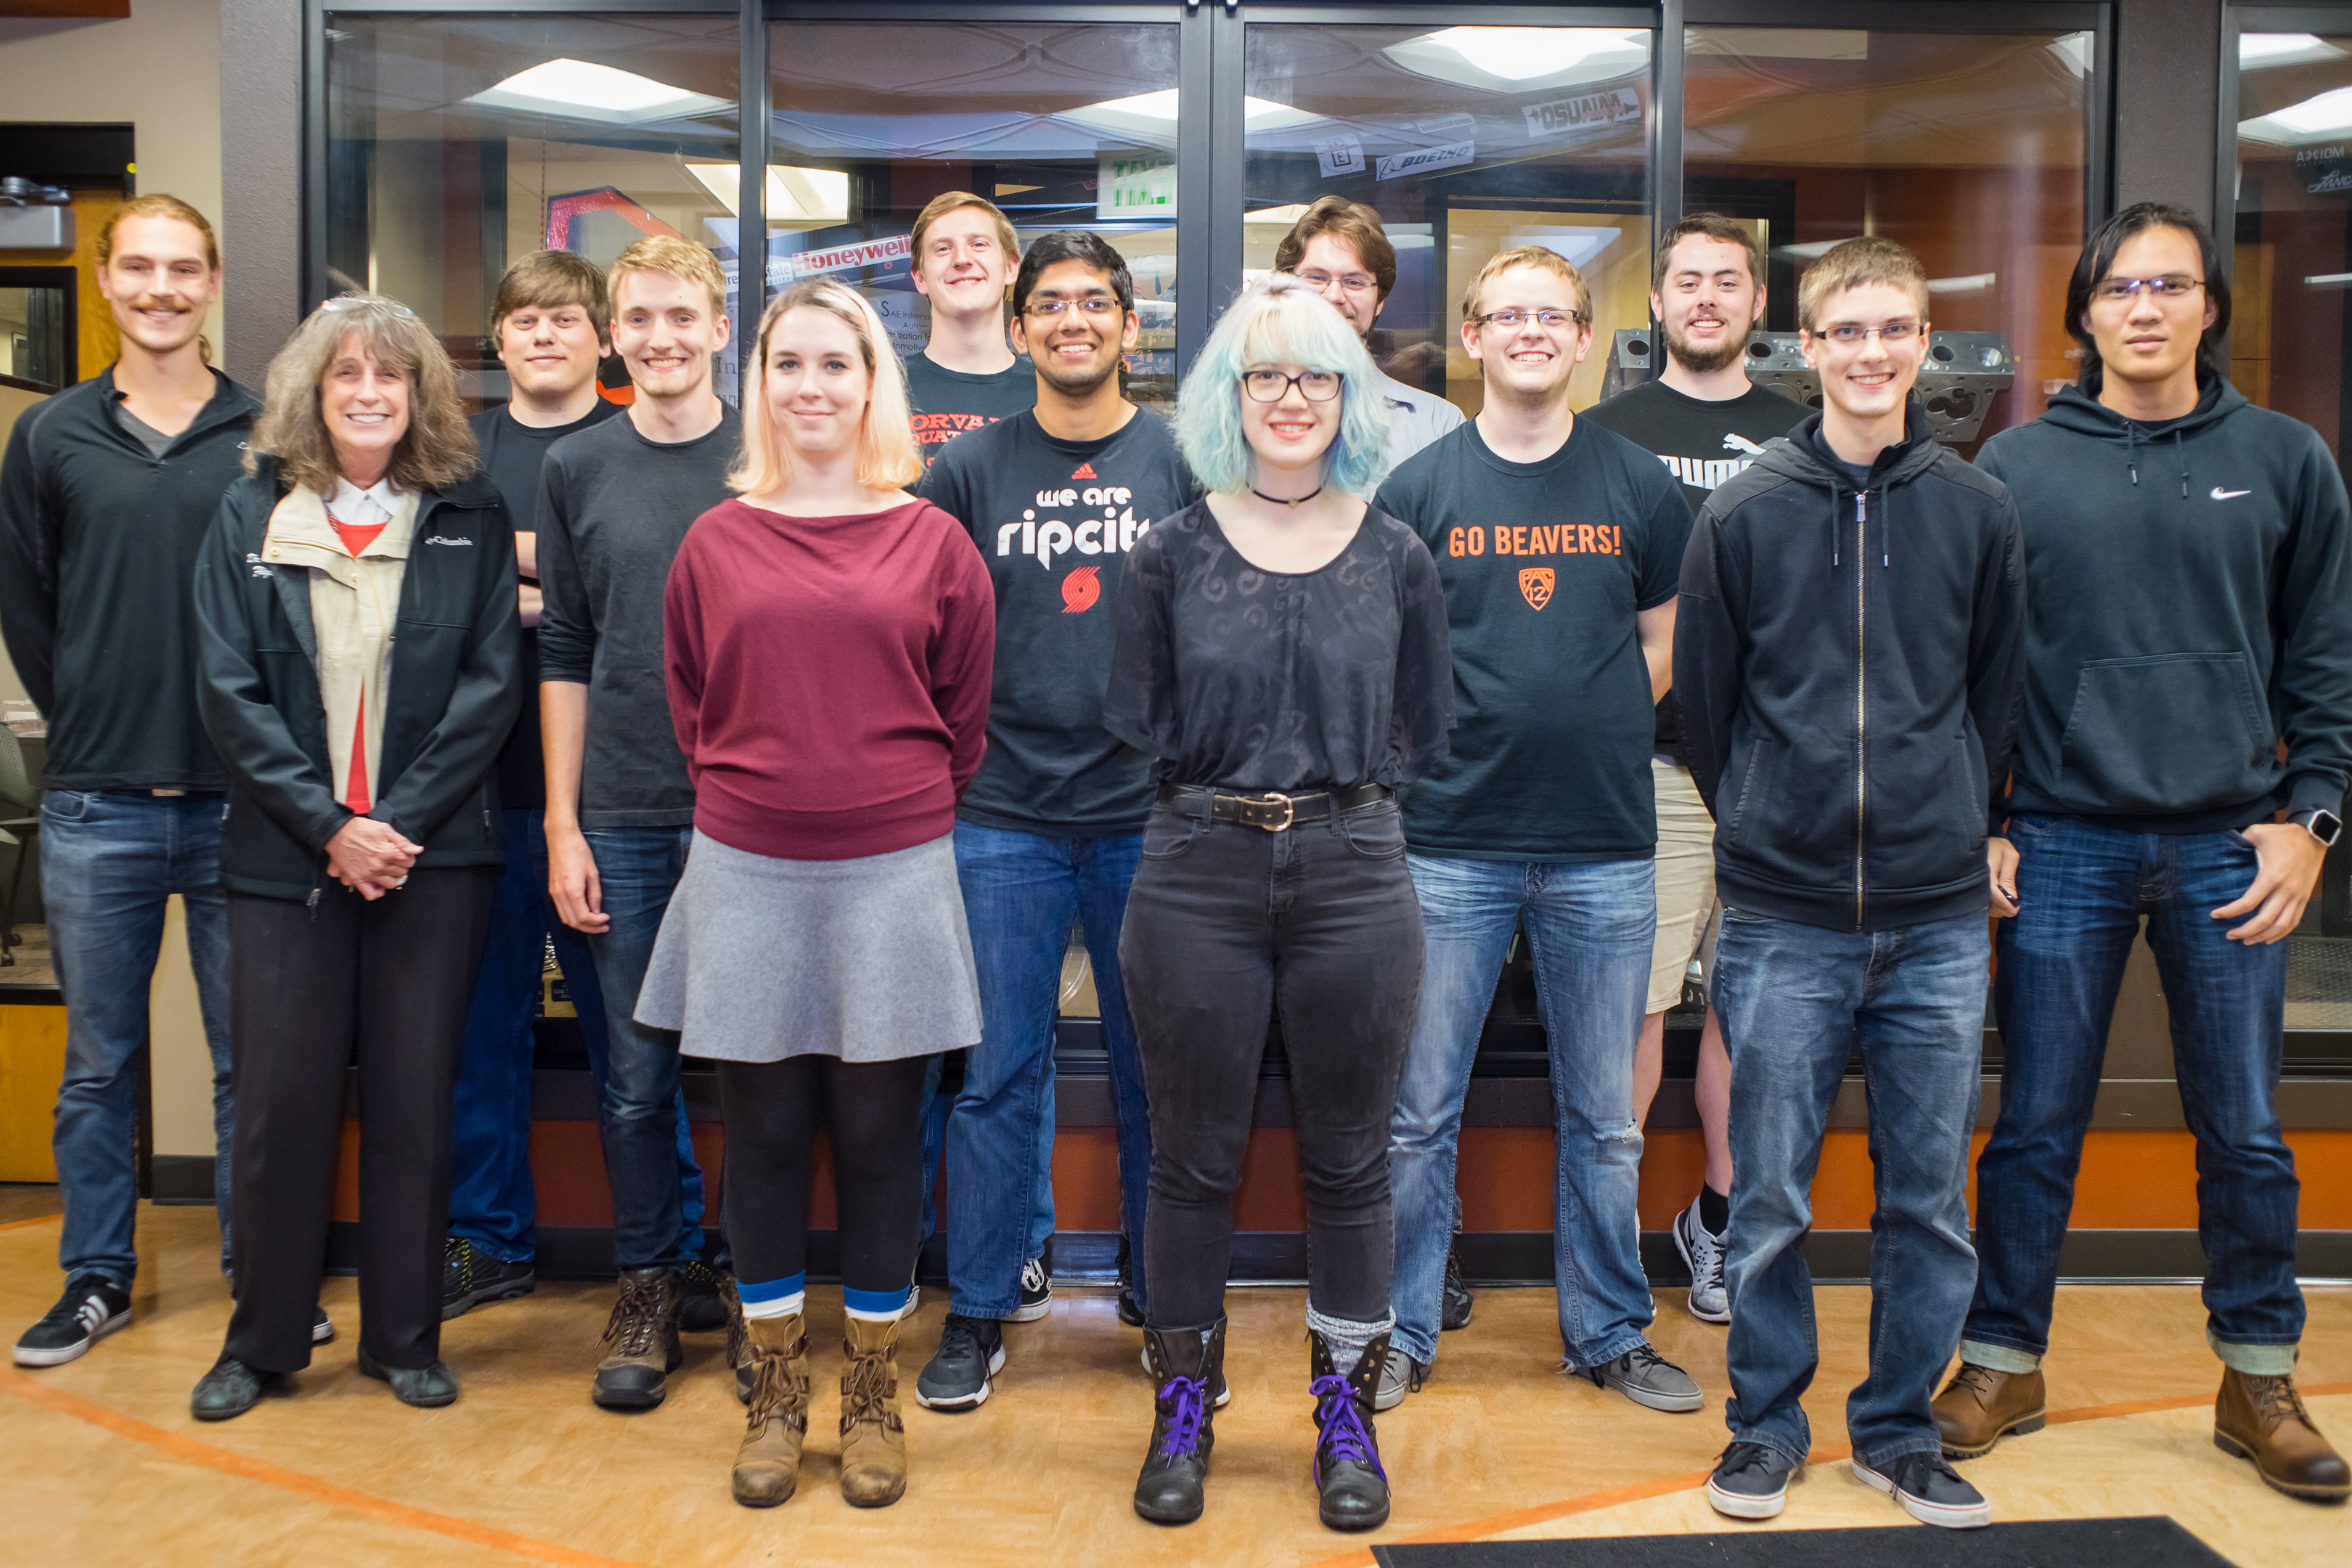
\includegraphics[width=\textwidth]{./images/AllTeam}
\begin{center}
From left to right,
\end{center}

\subsubsection{Software Team Photo}
\begin{center}
From left to right, Michael Humphrey, Helena Bales, Amber Horvath, and James
\end{center}

\subsection{CAD Models}
CAD Models created by the Mechanical Engineering teams of Hephaestus.
\subsubsection{Front View}
\includegraphics[width=\textwidth]{./images/CAD/FRONT}
\subsubsection{Back View}
\includegraphics[width=\textwidth]{./images/CAD/BACK}
\subsubsection{Right View}
\includegraphics[width=\textwidth]{./images/CAD/RIGHT}
\subsubsection{ISO 1 View}
\includegraphics[width=\textwidth]{./images/CAD/ISO_1}
\subsubsection{ISO 2 View}
\includegraphics[width=\textwidth]{./images/CAD/ISO_2}
\subsubsection{ISO 3 View}
\includegraphics[width=\textwidth]{./images/CAD/ISO_3}
\subsubsection{ISO 4 View}
\includegraphics[width=\textwidth]{./images/CAD/ISO_4}
\subsubsection{Left View}
\includegraphics[width=\textwidth]{./images/CAD/LEFT}
\subsubsection{Left Fully Deployed View}
\includegraphics[width=\textwidth]{./images/CAD/LEFT_DEPLOYED_FULL}
\subsubsection{Top View}
\includegraphics[width=\textwidth]{./images/CAD/TOP}
\subsubsection{Top Deployed View}
\includegraphics[width=\textwidth]{./images/CAD/TOP_DEPLOYED}
\subsubsection{Top Deployed Angle View}
\includegraphics[width=\textwidth]{./images/CAD/TOP_DEPLOYED_ANGLE}
\subsubsection{Top Fully Deployed View}
\includegraphics[width=\textwidth]{./images/CAD/TOP_DEPLOYED_FULL}

\subsection{Electrical Schematics}
Electrical Schematics created by the Electrical Engineering teams of Hephaestus.
\subsubsection{Voltage Regulator}
\includegraphics[width=\textwidth]{./images/EESchems/voltageRegulator}
\subsubsection{Motor Driver}
\includegraphics[width=\textwidth]{./images/EESchems/motorDriver}
\subsubsection{AVR}
\includegraphics[scale=.4]{./images/EESchems/AVR1}
\includegraphics[scale=.4]{./images/EESchems/AVR2}

\includegraphics[scale=.4]{./images/EESchems/AVR3}

\subsection{Power Budget}
\includegraphics[width=\textwidth]{./images/OtherDocs/powerBudget}

\subsection{Mass Budget}
\includegraphics[width=\textwidth]{./images/OtherDocs/massBudget}

\subsection{Pin Assignments}
\subsubsection{Power Pin Assignment}
\includegraphics[width=\textwidth]{./images/OtherDocs/powerPinAssignments}
\subsubsection{Telemetry Pin Assignment}
\includegraphics[width=\textwidth]{./images/OtherDocs/telemetryPinAssignments}

\subsection{Timer Events}
\includegraphics[width=\textwidth]{./images/OtherDocs/timerEvents}

\subsection{Payload Placement}
\includegraphics[width=\textwidth]{./images/OtherDocs/placement}

\subsection{Launch Compliance}
\includegraphics[width=\textwidth]{./images/OtherDocs/userGuideCompliance}

\subsection{Budget}
\includegraphics[width=\textwidth]{./images/OtherDocs/budget}


\section{Glossary}
\glsaddall
\printglossaries

\end{document}
